\documentclass[12pt,oneside]{jsbook}
\bibliographystyle{junsrt}
\usepackage{amsmath,amsthm,amssymb}
\usepackage{arydshln}
\usepackage{multicol}
\usepackage[dvipdfmx]{graphicx}
\usepackage{comment}
\usepackage{bm}
\usepackage{caption}
\newcommand{\argmax}{\mathop{\rm arg~max}\limits}
\newcommand{\argmin}{\mathop{\rm arg~min}\limits}
\usepackage{epsfig}
%\setlength{\textheight}{186mm}
\setlength{\columnseprule}{0.3pt}
\begin{document}
\pagestyle{empty}
\begin{center}
\vspace*{3cm} \underline{\HUGE 修士論文} \\
\vspace{0.5cm}
\bf{
\Huge 1次元アレイアンテナ式地雷可視化\\
\Huge システムにおける縦縞ノイズの軽減}\\
\vspace{0.5cm}
\huge 平成29年2月3日提出 \\
\vspace{3cm}
\huge 指導教員 \hspace{5cm} 廣瀬 明 教授 \\
\vspace{2cm}
\Large 東京大学大学院工学系研究科電気系工学専攻 \\
\vspace{1cm}
\huge 37-156465 \hspace{3cm} 小山 英利香
\end{center}


\newpage 
\setcounter{page}{1}
\pagestyle{headings}
\tableofcontents

\newpage 
\chapter{序章}
\section{研究背景}
\subsection{地中探査レーダによる地雷探査}
電磁波を用いた地中探査レーダ(Ground-Penetrating Radar:GPR)は探査対象へ
の非接触かつ非破壊な探知が可能なため,埋設物探査や地下水調査など多くの分野で
用いられている\cite{Arai}\cite{2007TCounts}.同様に,非金属で製作された地雷の探査に
も活用できる技術として,広く研究の対象となっている\cite{chichi}\cite{JeroenYarovoy}\cite{YaroboyLighthart}\cite{2004MSato}
\cite{2005Sato}\cite{2009Sato}.

しかしGPRを用いた地雷探査には以下の難点がある.
\begin{enumerate}
\item 対象となる対人地雷が小型である
\item 金属に比べてプラスチックの反射率が低い
\item 地中の浅い部分を探査するために地表面の影響が大きい
\item ほかの散乱体が同時に存在する
\end{enumerate}
これらの要因により,散乱波の位相と振幅のデータだけで
埋設された地雷を直接特定することは難しい.
\subsection{地雷可視化システム}
先述の問題に対して,本研究室ではGPRの散乱波により得られた地雷に特有のテクスチャ
の特徴量を複素自己組織化マップ(Complex-valued Self-Organizing Map : CSOM)
によって特定することで,地雷を可視化するシステムを実現させた
\cite{2007SMas}\cite{2008SMas}\cite{2009Nakano}\cite{2010Nakano}.

本システムにおける地雷可視化のプロセスは,以下に示す様に4段階に分けられる.
\begin{enumerate}
 \item マイクロ波送受信のフロントエンドにより地表面からの散乱波データを取得する
 \item 取得されたデータに前処理をして複素テクスチャ特徴量ベクトルを計算,抽出する
 \item 抽出されたテクスチャ特徴量ベクトルをCSOMにかけて適応的に分類する
 \item 区分化された特徴量に対して図\ref{so1mine}のように地雷らしさを評価する
\end{enumerate}
ベクトルネットワークアナライザがマイクロ波を発生させ,多段に組まれたスイッチの
切り替えにより1つのアンテナにマイクロ波が導かれ送信される.散乱波
は別の1つのアンテナが受信し,多段スイッチを通ってベクトルネットワークアナラ
イザで観測される.
取得したデータはノート型パーソナルコンピュータに転送され,そこで解析が行
われる.

しかし,本システムには
\begin{enumerate}
 \item 高周波用コネクタが多くメンテナンスに時間がかかる
 \item メカニカルスイッチの反復使用で寿命が短い
 \item 21cm*14cmの面積計測に22分必要と,時間がかかる
 \item アンテナを密に配置しているため直接結合の影響が大きい
\end{enumerate}
という課題が残されていた.
\begin{figure}[t]
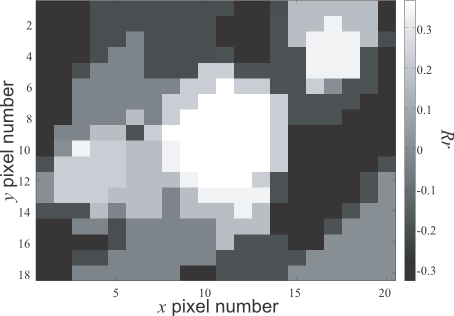
\includegraphics[width = \hsize]{so1mine.png}
\caption{地雷らしさの表現}
\label{so1mine}
\end{figure}

\section{目的}
本研究では上記課題を解決する
新しいシステムを用いて実際に地中を測定し,自己組織
化マップを適用して従来の2次元アレイアンテナ式地雷可視化システムと遜色な
く地雷を可視化することを目標とする.
本稿では新型となる1次元アレイアンテ
ナ式地雷可視化システムについて,新しいフロントエンドの
構造に起因する縦縞ノイズ問題
を,ハードウェア面・ソフトウェア面で解決する手法を提案する.

\newpage
\chapter{地雷可視化システム}
\section{従来のフロントエンド}
\subsection{システムの概要}
2次元アレイアンテナ式地雷可視化システムの概要を図~\ref{pic:const_ov}に示す.
システムはアンテナ部,スイッ
チング部,画像処理部から構成されている.
フロントエンドはタワー状になっており,底面にアンテナが取り付けられ
ていたため,フロントエンドを持ち上げて計測したい地表の真上に持って
いく必要があり,重量もあるために危険を伴った.
\begin{figure}[hbtp]
\begin{center}
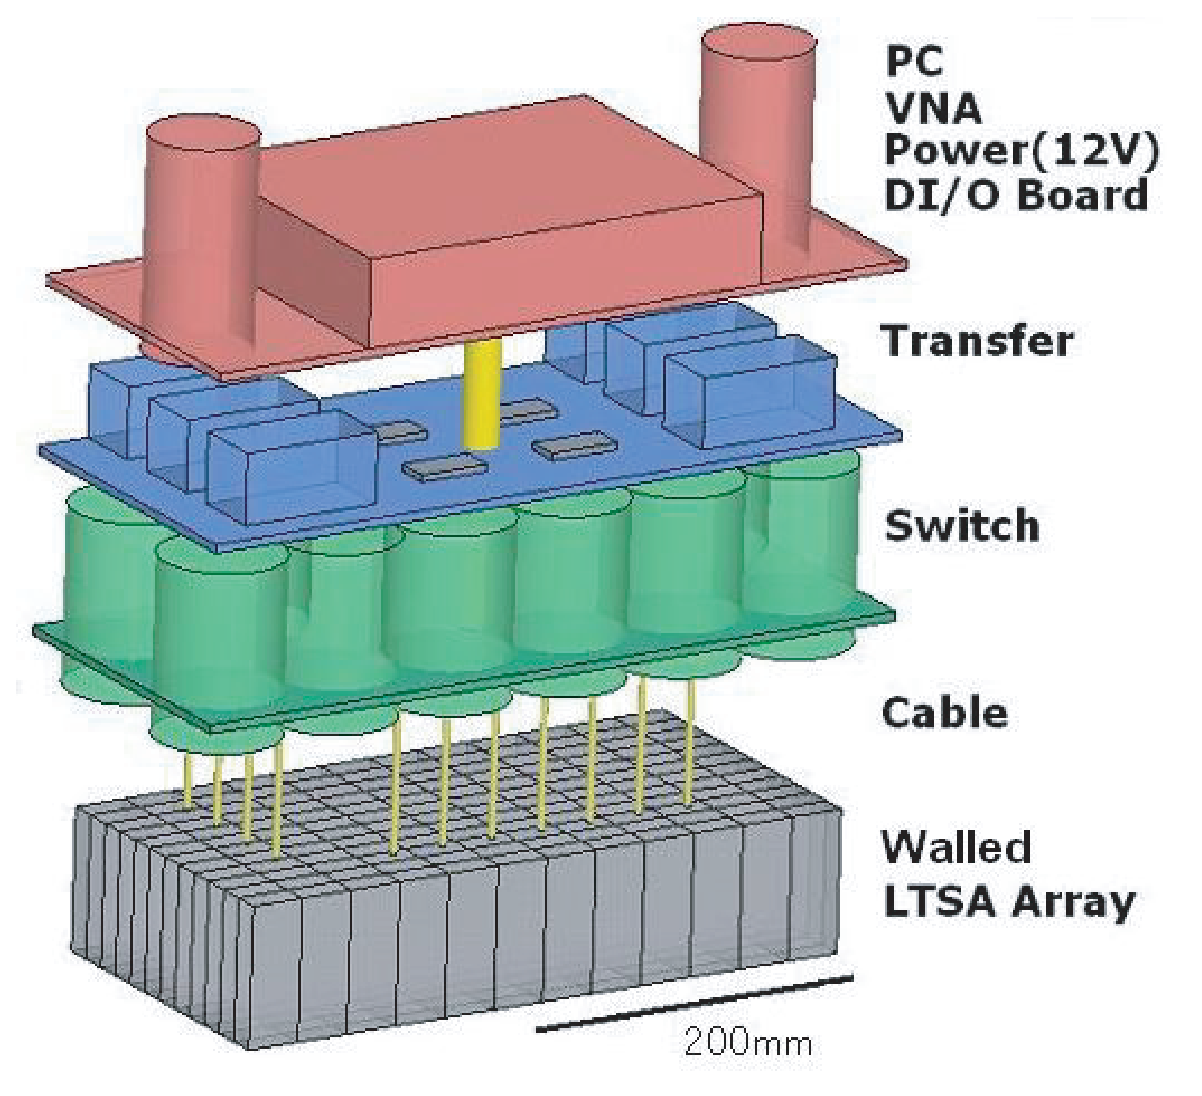
\includegraphics[width = \hsize]{so1.eps}
\caption{2次元アレイアンテナ式地雷可視化システムの概要図} \label{pic:const_ov} 
\end{center}
\end{figure}

アンテナ部は図~\ref{pic:transmit}のように構成される.
エレメントにはWalled Linearly Tapered Slot Antenna
 (Walled LTSA)\cite{2007SMas}が使われている.
このアンテナは高指向性,軽直接結合,
広帯域かつ高ゲインであり,近接場イメージングに適
している.このシステムにおいてGPRに用いる周波数帯は8$\sim$12[GHz]で,8[G
Hz]から0.4[GHz]刻みで散乱波を取得する.
アンテナ部はこのアンテナを12個ずつ2次元に144個並べた
構造をしている.
しかし,このアンテナが軽直接結合といっても,影響を無視することはできなかった.

\begin{figure}[hbtp]
\begin{center}
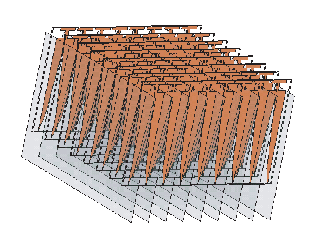
\includegraphics[width=\hsize]{LTSA.eps}
\caption{アンテナ部の全体図} \label{pic:transmit} 
\end{center}
\end{figure}
ベクトルネットワークアナライザで発生させたマ
イクロ波を多段スイッチングで指定したアンテナから送信する.マイクロ波が地表や
地中の散乱体により散乱し,この散乱波を同じく多段スイッチングで指定したアンテ
ナで受信する.受信したデータはベクトルネットワークアナライザからコンピュー
タに送られる.散乱波は$x$,$y$の空間的2次元領域と周波数領域の3次元の
データになっており,これを散乱画像として扱う.画像処理部では
測定データをSelf-Organizing Map(SOM)によって処理し,適応的に区分化する.
更に既知の地雷画像と比較し,地雷らしさを算出する.
\subsection{従来のフロントエンドの問題点}
本システムの課題について詳細に述べる.
まず,メンテナンスに非常に時間がかかる.
配線が増えるとコネクタ
部の故障に対応する手間も増えるためである.
また,本システムには信号の減衰が少ない理想的なスイッチ
である高周波用のメカニカルスイッチ20個が多層化されて用いられ,これがさ
まざまな送受信の組み合わせを可能にしている\cite{2008SMas}
.しかし,機械式であるために電子スイッチに比べ反復使用で壊れやすいという難点
もあった.同時に,機械式スイッチは切り替えに時間がかかり,上記505点の計
測に22分を要していた.
さらに高密度にアンテナを配置しているため,直接結合の影響を物理
的に極力排除することを考えたWalled LTSAでも,実際には直接結合の影響が無
視できないほど大きく出ていた.
これらの問題を回避するために,新しいフロントエンドが提案された.

\newpage
\section{以前提案した1次元アレイアンテナ式地雷可視化システム}\label{1array_before}
前節で提案されたと述べた1次元アレイアンテナ式地雷可視化シ
ステム\cite{ejiri}は,図\ref{so2}のように,以下のコンポーネントによって構成される.
\begin{enumerate}
\item 1次元アレイアンテナによるフロントエンド
\item 下層の電子式スイッチ
\item 上層のメカニカルスイッチ
\item ベクトルネットワークアナライザ
\item アーム・アクチュエータ
\item パーソナルコンピュータ
\end{enumerate}

フロントエンドにはTaper-Walled LTSA(図\ref{pic:twltsa}(b))が使われている.
このLTSAは我々の研究室で製作されたものであり,同じく以前我々の研究室から
提案したWalled LTSA(図\ref{pic:twltsa}(a))よりも更に直接結合が軽減されて
いる\cite{2011Nakano}.
\begin{figure}[btp]
 \begin{center}
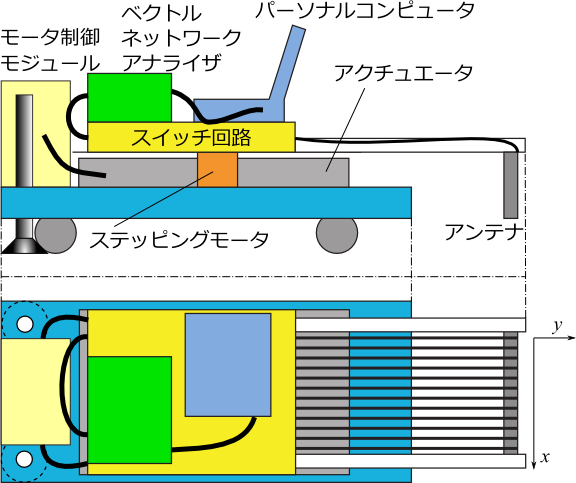
\includegraphics[width =\hsize ]{so2-2.png}
\caption{1次元アレイアンテナ式地雷可視化システム}
\label{so2}
  \end{center}
\end{figure}
\begin{figure}[btp]
\begin{center}
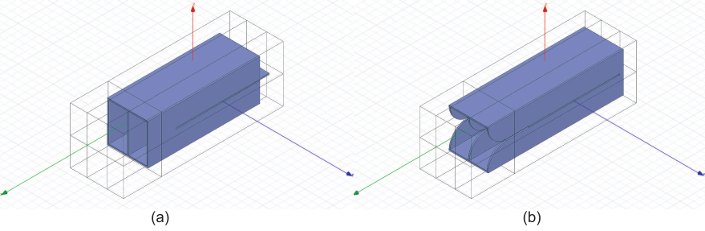
\includegraphics[width =\hsize]{walled-taper.png}
\caption{Walled LTSAとTaper-Walled LTSA} \label{pic:twltsa} 
\end{center}
\end{figure}
アンテナを1列に配置することにより,アンテナ数を144から12に,
メカニカルスイッチ数を20から5に減らした.配線数,高周波用コネク
タの数を大幅に削減することができ,保守性が向上した.
また,メカニカルスイッチの数を減らしたため,故障率が下がり,
信頼性も向上したと考えられる.

スイッチングの高速化のために,
このシステムのスイッチング回路には一部pinダイオードスイッチが使用されて
いる(図\ref{scircuit}).pinダイオードとは一般のダイオードに用いられるP
層とN層の間に真性半
導体のI層がある3層構造となっているダイオードで,高周波におけるスイッチ
特性に優れているために一般に広く使われている.
しかしpinダイオードは信号の減衰
が大きいために,この多段式スイッチングシステムでは
高速かつ頻繁な切り替えが求められる下層の部分に
これを使用し,それほど切り替えが頻繁である必要がない
上層の部分にはメカニカルス
イッチを用いることで,信号の減衰を抑えつつ,計測時間を短縮し,長寿命化と
保守性の向上を目指した.

\begin{figure}[btp]
\begin{center}
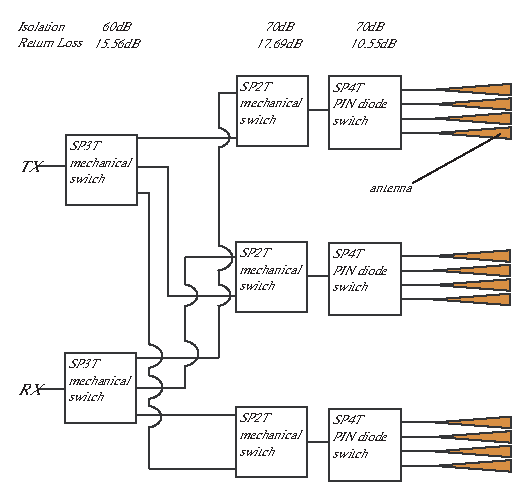
\includegraphics[width =\hsize ]{switch-circuit.eps}
\caption{スイッチング部の回路図}
\label{scircuit}
 \end{center}
\end{figure}

本システムでのデータ点の取り方は図\ref{so2get}のようになっている.
アンテナを1次元に配列し($x$方向データ点),
アクチュエータにより直交方向
($y$方向データ点)にアンテナを動かすことで,2次元に画像を取得できる.
従来のシステム
では送信アンテナに対し受信アンテナを1つ隣,2つ隣,1つ下,1つ斜め下とした
4種類505点のデータを取得したが,新型のシステムでは1つ隣,2つ隣の2種類のデー
タしか取れない.これでは一見して情報量が減少しているようだが,サーボを用いてアン
テナを自由に前後に動かせるため,実際には同程度の情報量を得ることができる.
実験では,一列のアンテナで21点の計測が可能であることを受けてサーボ
の進行方向にもアンテナの列長14.3cmと近い14.0cmの間に21点のデータを取ることとし,
441点のデータを得た.
\begin{figure}[btp]
 \begin{center}
 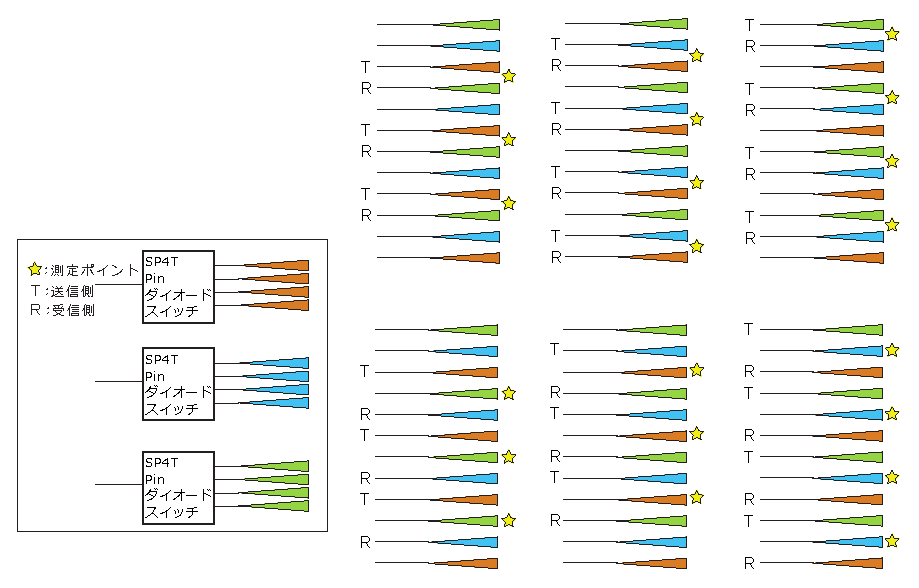
\includegraphics[width =\hsize ]{switch-circuit2.eps}
\caption{データ取得方法}
\label{so2get}
 \end{center}
\end{figure}

\newpage
\section{可視化処理}
\label{021920_15Feb15}
\subsection{前処理}
フロントエンドから得られるデータには,アンテナの個体差,使用するスイッチ
やケーブルの違いによる高周波経路差,アンテナ間の直接結合の3つのノイズの影響がある.
これらを補正するために,事前に補正用のデータを取得し
ておく.これにはアンテナを電波吸収体を敷いた床から90cm上げて
周囲に何もない状態で計測したものを用いる.
得られるデータは複素数$z_{raw}$,補正用のデータは$z_{coup}$である.
これに対し直接結合を以下の式に従い補正し,補正後のデータ$z_{after}$を得る.

\begin{equation}
 z_{tmp}(x,y,f)=z_{raw}(x,y,f)-z_{coup}(x,y,f)
\end{equation}
\begin{equation}
 z_{after}(x,y,f)=\exp(-i\theta_{path})\cdot\exp(-i\angle z_{coup}(x,y,f))\cdot z_{tmp}(x,y,f)
\end{equation}
\begin{equation}
 \theta_{path}=\frac{2\cdot2\pi}{\lambda} \sqrt{d^2+h^2}
\end{equation}
ここで,$d$,$h$とは図\ref{dc}に示した部分の長さである.ただし$h$は
実際には分からないため,地表までの距離である4cmを採用した.
なお従来は,振幅の減衰差はそれほどないものとし,位相にのみ直接結合の補正
を行なっていた.
\begin{figure}[btp]
\begin{center}
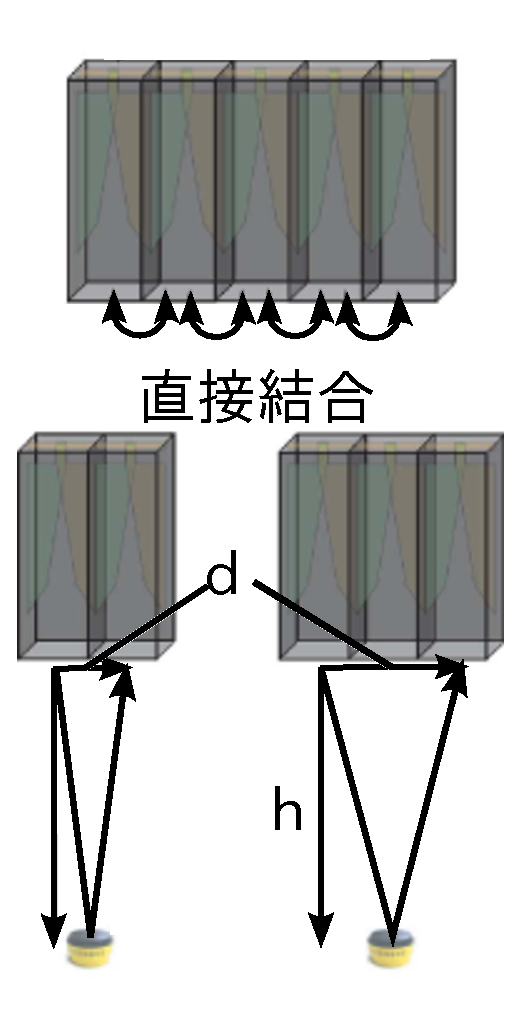
\includegraphics[width =0.5\hsize ]{directcoup.eps}
\caption{直接結合と補正のための経路長}
\label{dc}  
\end{center}    
\end{figure}

\begin{figure}[btp]
\begin{center}
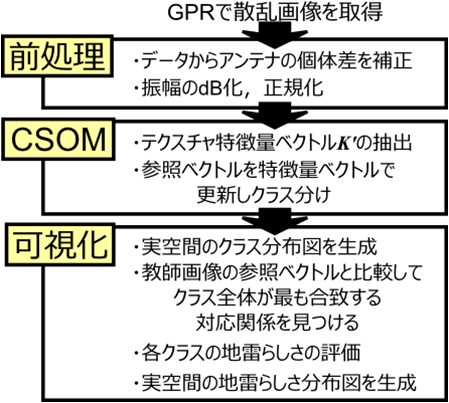
\includegraphics[width =0.8\hsize ]{flowchart.png}
\caption{データ取得から地雷可視化までの流れ}
\label{flow}
\end{center}        
\end{figure}

直接結合の補正の後,振幅をlogスケールにしてdBで表して人間の目の感覚に近づけ,
それを正規化
する.ここまでを前処理とし,これによって得られたデータをSOMに掛けて
区分化を行う.
\subsection{CSOM}
自己組織化マップ(SOM)とは,教師なしで適応的にデータを区分化する
ニューラルネットワークを用いた手法のことで,
与えられた入力情報の類似度を
マップ上の距離で表現するモデルである.

SOMは複数のニューロンで構成される.各ニューロンは入力ベクトルと同次元の
参照ベクトルを持つ.
SOMに入力ベクトルとなる特徴量ベクトルが与えられると,特徴量ベクトルに
最も近い参照ベクトルを持
つニューロンが勝者となる.このとき,座標空間上でより勝者の近くに位置する
ニューロンほど強く学習し,その強さに応じて自身の参照ベクトルを特徴量ベクト
ルに近づける.このように参照ベクトルの更新を繰り返し,ベクトル空間上での
参照ベクトル同士の関係性が座標空間上で表現される.

本システムでは,ニューロンを1次元のリン
グ状に配置したRing-SOMを用いる.また,複素数のデータを扱うため,複素数に
対応し,コヒーレントなデータに感受性を持っ
たSOMであるCSOM(Complex-valued SOM)を利用している
.今回は電磁波を扱うので,データがコヒーレンスを持つことが予想される.
測定データから特徴量ベクトルを抽出し,SOMを利用して各ピ
クセルの類似度を1次元の値として表現する.
区分化にあたっては,リング状のトポロジを用いて,8つのクラスを円形に配置し,
最も入力ベクトルに近いベクトルを持つ勝者クラスを$\alpha$で強化し,その両隣の
クラスを$\alpha$よりも弱い$\beta$で強化する.

\subsection{特徴量ベクトルの抽出}
CSOMでは局所的テクスチャを見て分類する.
まず,$L\times L$ピクセルの局所ウィンドウを設定して,
テクスチャ特徴量を抽出する.
今回は$L=4$としている.
その後,$(x,y)$について掃引し,特徴量ベクトル${\bm K}(x,y)$を次のように得る.
\begin{eqnarray}
{\bm K} = \left[\begin{array}{ccc}
      {\it K_{{\rm m}}} & {\bm K_{{\rm s}}} & {\bm K}_{{\rm f}}
           \end{array} \right]^{\mathrm{T}}\label{eq.K}
\end{eqnarray}
ただし$T$は転置を表す.
位置$(x,y)$における${\bm K}(x,y)$は,空間的なテクスチャ特徴量
${\it K_{{\rm m}}},{\bm K_{{\rm s}}}$と周波数領域のテクスチャ特徴量
${\bm K_{{\rm f}}}$からなる.
空間的なテクスチャ特徴量は,
各$(l_x,l_y)$の複素画素値の平均${\it K_{{\rm m}}}$,$(l_x,l_y)$の自己相関
${\it K_{{\rm s}}}(0,0)$,$(l_x,l_y)$と$(l_x,l_y+1)$,$(l_x+1,l_y)$,
 $(l_x+1,l_y+1)$との相互相関${\it K_{{\rm s}}}(0,1),
 {\it K_{{\rm s}}}(1,0),{\it K_{{\rm s}}}(1,1)$をとる.

\begin{eqnarray}
{\bm K_{{\rm s}}} = \left[\begin{array}{cccc}
 {\it K_{{\rm s}}}(0,0) & {\it K_{{\rm s}}}(0,1) &
 {\it K_{{\rm s}}}(1,0) & {\it K_{{\rm s}}}(1,1)
 \end{array} \right]^{\mathrm{T}}
\end{eqnarray}

ただし,$l_x,l_y$は局所ウィンドウの中の座標であり,$N$は周波数領域で使用
する画像の数,$f_0$は使用した最も低い周波数である.
 また周波数領域での特徴量として,$f_{\rm int}$
 高い周波数での同じ位置との相互相関${\bm K_{{\rm f}}}$をとる.

 \begin{eqnarray}
  {\bm K_{{\rm f}}} = \left[\begin{array}{ccc}
                      {\it K_{{\rm f}}}(1) & \ldots & {\it K_{{\rm f}}}(n)
                            \end{array} \right]^{\mathrm{T}}
 \end{eqnarray}
 \begin{eqnarray}
{\bm K_{{\rm f}}}(n) = \frac{1}{L^2}\sum_{l_x = 1}^{L}\sum_{l_y =
 1}^{L}&z^{\dagger}&\left(l_x, l_y, f_0+(n+1)f_{{\rm int}}\right)
 \nonumber\\&&\hspace{0em}\cdot
 z\left(l_x, l_y, f_0+nf_{{\rm int}}\right)
\end{eqnarray}

これらの特徴量を式(\ref{eq.K})のように1つのベクトルにまとめている.

\subsection{地雷クラスの同定}
以上から得られた特徴量ベクトルをSOMに代入し,参照ベクトルを更新して学習
を行う.最終的に生成されたSOMはクラスごとに色分けされた区分画像と
なっている.実
際の地雷可視化作業では,地雷クラスを持つ教師画像を複数用意し,この未知の
区分画像と照らし合わせることで,未知の区分画像の地雷らしさを評価する\cite{2010Nakano}.
本稿では,この教師画像を用意するために正しく地雷クラスを検出できるこ
とを提示する.

なお,空間特徴量と周波数特徴量を分けてそれぞれCSOMにかけ,それらの相互相
 関により可視化するという手法もある\cite{ejiri}が,今回は
計算の高速化のため採用していない.
\newpage
\section{異方性を軽減する自己組織化マップ}
\subsection{異方的重み付け}
一次元アレイアンテナ式のフロントエンドから得られる散乱画像
により地雷を可視化する時,
後述するように
縦縞の影響を抑えて地雷を可視化する必要が生じた.
そこで,縦方向の変化に敏感になるようにCSOMの自己組織化ダイナミクスに異方
性をとり入れた.(発表文献\cite{koyama})

まず,全ての$(x,y)$について特徴量ベクトルの分散共分散行列$\Sigma$を算出する.
次に,特徴量ベクトルの要素のうち異方性があると判明しているものを選定する.
今回は,$K_{{\rm s}}(0,1)$,
$K_{{\rm s}}(1,0)$,
$K_{{\rm s}}(1,1)$
の3要素の間に異方性があると考えた.$\Sigma$からこの3要素同士の共分散行列
$\Sigma_3$を抽出
し,行列${\Sigma_w}^{-\frac{1}{2}}$を取得する.これを用いて重み
付けを行う.

\begin{equation}
\Sigma_w = \left(\begin{array}{c:c:c}
	   I_2&\Large{0} &\Large{0} \\
\hdashline %
\Large{0} &\Sigma_3& \Large{0}\\
\hdashline %
\Large{0}&\Large{0} &I_9
		\end{array}
\right) 
\end{equation}

勝者クラスを決定する際に従来はユークリッド距離を用いていた.
\begin{equation}
\tilde{c}_E = \argmin_{c} \|{\bm K} - {\bm w_c} \|\label{192027_15Feb15}
\end{equation}
これを重み付けすると,${\Sigma_w}^{-\frac{1}{2}}$はエルミート行列であるの
で以下のように変形できる.
\begin{eqnarray}
\tilde{c}_E&=&\argmin_{c} \|{\Sigma_w}^{-\frac{1}{2}}\left({\bm K} -
						      {\bm w_c}\right)\|\\
 &=&\argmin_{c} \sqrt{\left({\Sigma_w}^{-\frac{1}{2}}\left({\bm K} -
						      {\bm w_c}\right)
		      \right)^{\dagger}
                \left({\Sigma_w}^{-\frac{1}{2}}\left({\bm K} - {\bm
						w_c}\right)\right)}\\
 &=&\argmin_{c} \sqrt{\left({\bm K} - {\bm w_c}\right)^{\dagger}
    {\Sigma_w}^{-1}\left({\bm K} - {\bm w_c}\right)}
\end{eqnarray}
この式から分かるように,異方性のある要素においてはユークリッド距離ではな
くマハラノビス距離となっている.従って,従来手法において異方的重み付けす
る場合,マハラノビス距離を勝者クラスの決定に用いることとなる.
マハラノビス距離とは,分布する2つの確率変数ベクトル${\bm x},{\bm y}$とその
共分散行列$\Sigma$を用いて
\[
 d({\bm x},{\bm y}) = \sqrt{\left({\bm x}-{\bm
 y}\right)^T\Sigma^{-1}\left({\bm x}-{\bm y}\right)}
\]
で表される距離である.共分散行列の逆行列をかけることで,楕円形の分布を正円
形に歪ませて,情報量を補正するものである.図\ref{maha}において,ユークリッド距離で
は$a>b$であるのに対し,マハラノビス距離では$a<b$とすることができる.

\begin{figure}[btp]
 \begin{center}
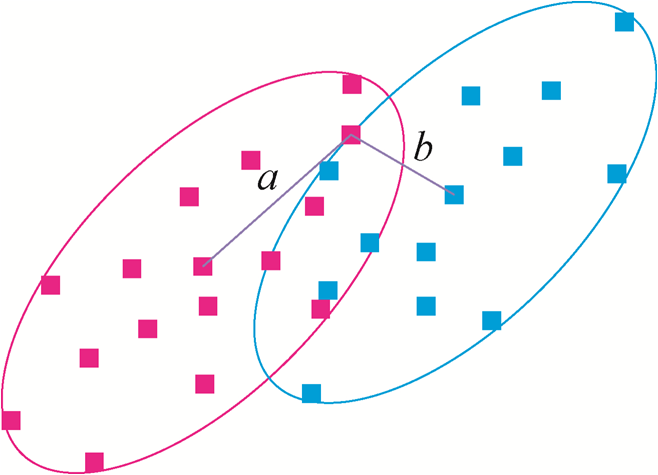
\includegraphics[width =\hsize ]{maha.png}
\caption{2つの変数ベクトルの分散と距離}
\label{maha}
  \end{center}
\end{figure}

%具体的には,特徴量ベクトルを異方的に重み付けし,次のように$(l_x,l_y+1)$
%との相互相関に係数$C$を,$(l_x+1,l_y+1)$との相互相関に係数
%$D$をかける.
%
%\begin{eqnarray}
% {\bm K_{{\rm s}}'} = \left[
%\begin{array}{cccc}
% 1& & & \\
%  &C& & \\
%  & &1& \\
%  & & &D
%\end{array}
%                    \right]
% \left[
%  \begin{array}{c}
%   {\it K_{{\rm s}}}(0,0)\\
%   {\it K_{{\rm s}}}(0,1)\\
%   {\it K_{{\rm s}}}(1,0)\\
%   {\it K_{{\rm s}}}(1,1)
%  \end{array}
% \right]
%\end{eqnarray}
%
%これによって得られる特徴量ベクトル${\bm K'}$を
%新たな特徴量ベクトルとしてCSOMに入力する.
%\begin{eqnarray}
%{\bm K'} = \left[\begin{array}{ccc}
%      {\it K_{{\rm m}}} & {\bm K_{{\rm s}}'} & {\bm K_{{\rm f}}}
%           \end{array} \right]^{\mathrm{T}}
%\end{eqnarray}

\subsection{複素内積での勝者クラス決定法}
CSOMで各特徴量ベクトルの入力に対して勝者クラスを決定する方法には2通りある.
特徴量ベクトルと参照ベクトルのユークリッド距離をとり最小となるクラス
$\tilde{c}_E$を選択する方法(式(\ref{192027_15Feb15}))と,
特徴量ベクトルと参照ベクトルの複素内積を
とり最大となるクラス$\tilde{c}_I$を選択する方法\cite{2010Yoshida}である.
\begin{eqnarray}
\tilde{c}_I = \argmax_{c} \left( \left|
 \frac{{\bm K}^{\dagger}\cdot{\bm w_c}}{ \|{\bm K}\| \| {\bm w_c} \| }
                                   \right| \right)
\end{eqnarray}
従来の地雷可視化システムでは前者を選択していた.
しかし,コヒーレンスにより敏感な後者の方が有
効である\cite{aoyagi}.図\ref{ip}において,コヒーレンスのあ
る実線ベクトル(a)とコヒーレンスのない破線ベクトル(b)を扱う際,ユークリッド距離
による勝者クラス決定法では実部があるために実軸投射したときに大きい(b)が勝
者となる.しかし,コヒーレンスを重視する,複素内積による勝者クラス決定法
では,複素ベクトルのノルムが大きい(a)が勝者となる.

\begin{figure}[btp]
 \begin{center}
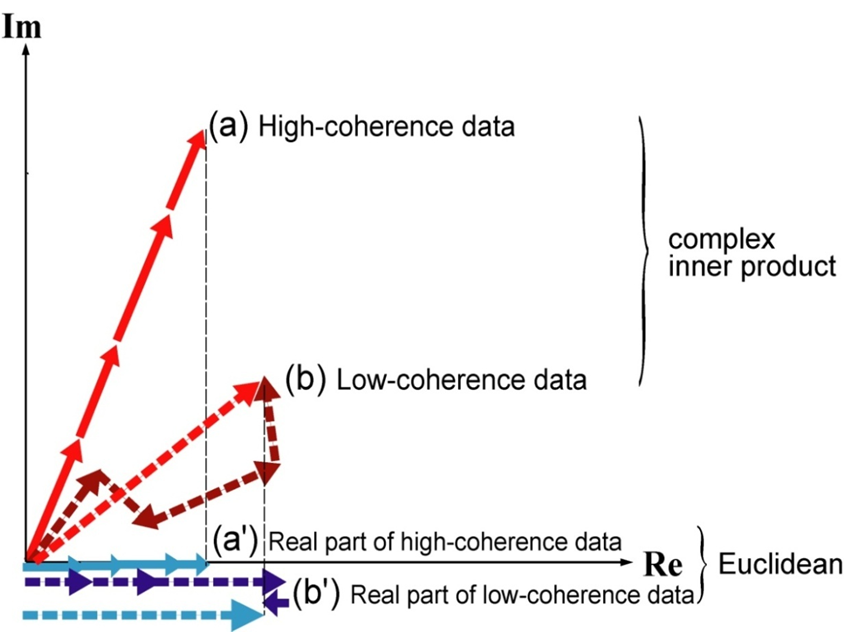
\includegraphics[width =\hsize ]{innerproduct.png}
\caption{複素内積が有利に働く場合}
\label{ip}
  \end{center}
\end{figure}

次に,本手法で前項で説明した異方的重み付けを行う場合の条件式を以下に表す.
\begin{eqnarray}
\tilde{c}_I &=& \argmax_{c} \left( \left|
\frac{\left({\Sigma_w}^{-\frac{1}{2}}{\bm K}\right)^{\dagger}\cdot
\left({\Sigma_w}^{-\frac{1}{2}}{\bm w_c}\right)
}{ \|{\Sigma_w}^{-\frac{1}{2}}{\bm K}\| \|{\Sigma_w}^{-\frac{1}{2}}{\bm w_c} \| }
                                   \right| \right)\\
 &=& \argmax_{c} \left( \left|
\frac{{\bm K}^{\dagger}{\Sigma_w}^{-\frac{1}{2}
\dagger}{\Sigma_w}^{-\frac{1}{2}}\cdot{\bm w_c}
}{ \sqrt{{\bm K}^{\dagger}{\Sigma_w}^{-1}{\bm K}}\sqrt{{\bm
w_c}^{\dagger}{\Sigma_w}^{-1}{\bm w_c}} }
                                   \right| \right)\\
 &=& \argmax_{c} \left( \left|
\frac{{\bm K}^{\dagger}{\Sigma_w}^{-1}\cdot{\bm w_c}
}{ \sqrt{{\bm K}^{\dagger}{\Sigma_w}^{-1}{\bm K}}\sqrt{{\bm
w_c}^{\dagger}{\Sigma_w}^{-1}{\bm w_c}} }
                                   \right| \right)
\end{eqnarray}

著者の卒業研究の結果,以上において,異方的重み付けと複素内積の組み合わせ
により,ユークリッド距離で勝者ベクトルを決定した時に比べ縦縞の
影響を排除して
地雷の形を検出できることが分かっている.
ユークリッド距離で勝者クラスを決定する手法により,異方的重み付けを行わずに
区分化した結果が図\ref{iso-e},
複素内積で勝者クラスを決定する手法により異方的重み付けを行った結果
が図\ref{aniso-i}である.

\begin{figure}[btp]
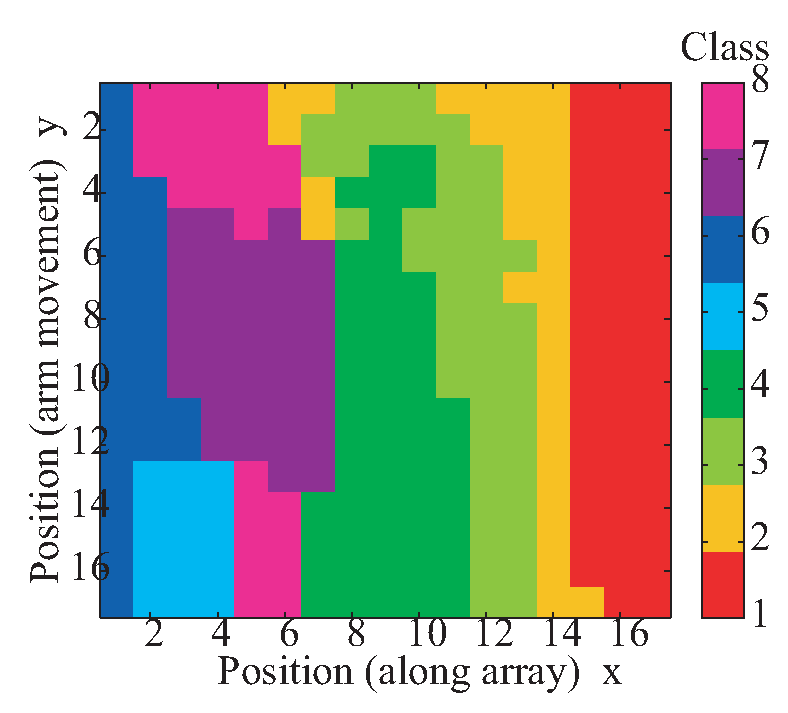
\includegraphics[width =\hsize ]{SOM_mine6_02005_e_raw.eps}
\caption{ユークリッド距離で勝者クラスを決定した時の異方的重み付けなしでの結果}
\label{iso-e}
\end{figure}

\begin{figure}[btp]
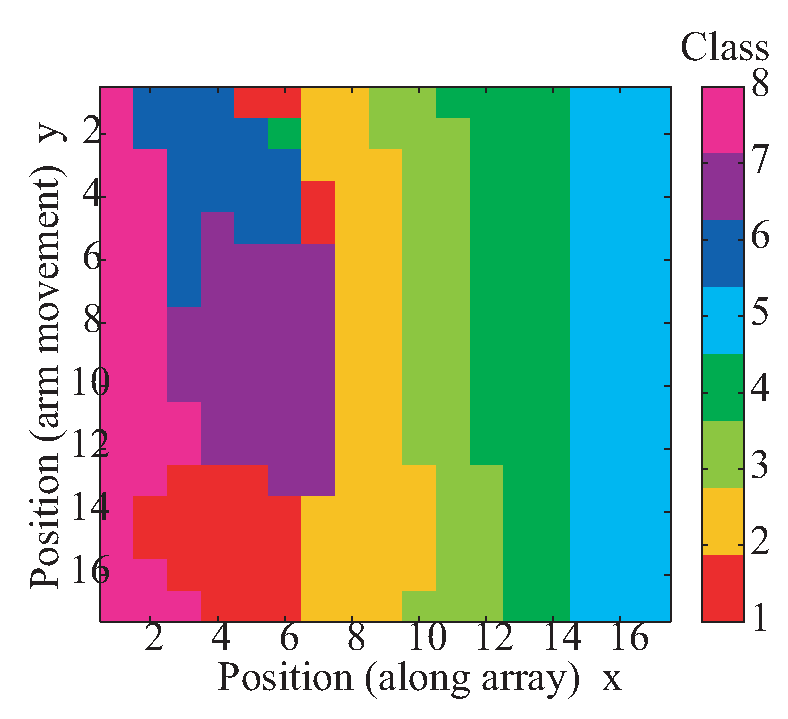
\includegraphics[width =\hsize ]{SOM_mine6_02005_i_wsqrt.eps}
\caption{複素内積で勝者クラスを決定した時の異方的重み付け結果}
\label{aniso-i}
\end{figure}

\newpage
\section{模擬地雷計測実験と縦縞ノイズ問題}

\subsection{計測方法}
図\ref{landmine}のように,外径40cmの立方体型の植木鉢を用意し,そこに渇い
た土を入れ模擬地雷
を埋設した.土には小石や小枝などの他の散乱源も多数存在している.フロント
エンドの高さはこの地面にほぼ接するような距離になっている.埋設する模擬地雷は
直径8cmの上面円形の形状をし,素材はプラスチックである.
\begin{figure}[hbtp]
 \begin{center}
 \includegraphics[width =0.8\hsize ]{landmine.png}
\caption{実験に用いた環境と模擬地雷埋設}
\label{landmine}
 \end{center}
\end{figure}
\subsection{計測結果}
図\ref{mine-raw}〜図\ref{direct-raw}は,GPRからベクトルネットワークアナライザを通じて得られた振幅と
位相のデータを補正前の段階で画像として表示したものである.アンテナの
個体差が縦縞となって表れているのが確認できる.図\ref{mine-raw}は模擬地雷を埋設した
地面を計測したもの,図\ref{none-raw}は地雷を埋設せずに地面を計測したもの,図\ref{direct-raw}は
アンテナ下90cmに何も遮るものがなく,かつその下に電波吸収体を敷いた空間を計測したものである.

この電波吸収体を計測したデータを直接結合の補正として用いてdata6を補正
した結果が図\ref{mine6-hosei}である.前処理では縦縞を軽減することはでき
るものの,完全に除去することはできないことが分かる.
\begin{figure}[hbtp]
 \begin{center}
     \begin{minipage}[c]{\hsize}
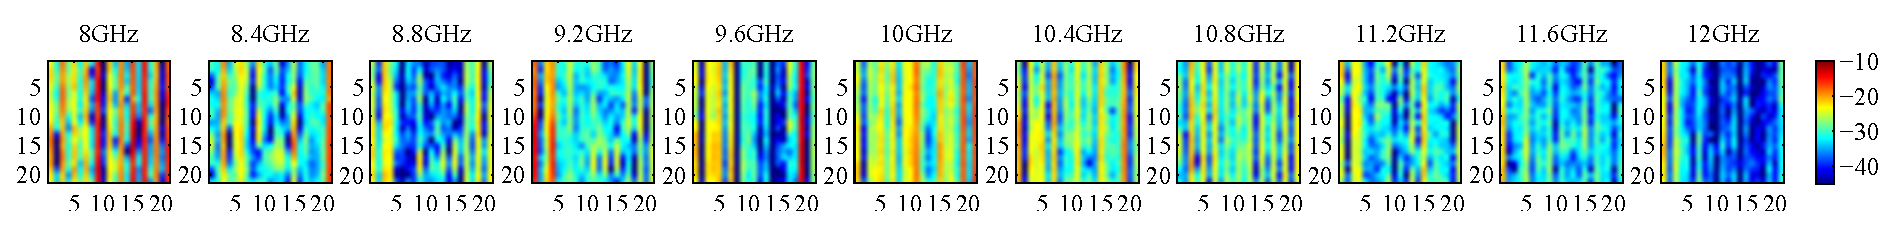
\includegraphics[width = \hsize ]{20150204_mine1_raw_a.eps}
\centering\textmd{data1,振幅}
  \end{minipage}
\\
     \begin{minipage}[c]{\hsize}
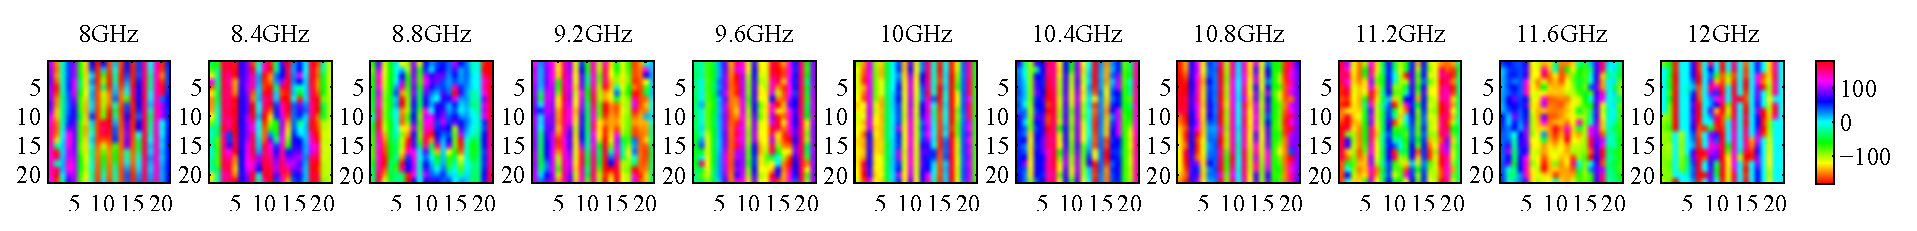
\includegraphics[width =\hsize ]{20150204_mine1_raw_p.eps}
\centering\textmd{data1,位相}
  \end{minipage}
\end{center}
\end{figure}
\begin{figure}[bhtp]
 \begin{center}
     \begin{minipage}[c]{\hsize}
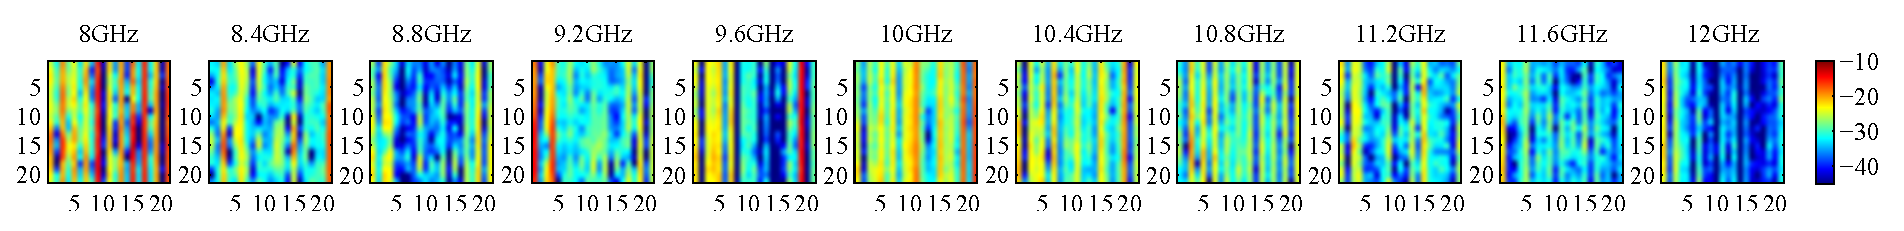
\includegraphics[width = \hsize ]{20150204_mine2_raw_a.eps}
\centering\textmd{data2,振幅}
  \end{minipage}
\\
     \begin{minipage}[c]{\hsize}
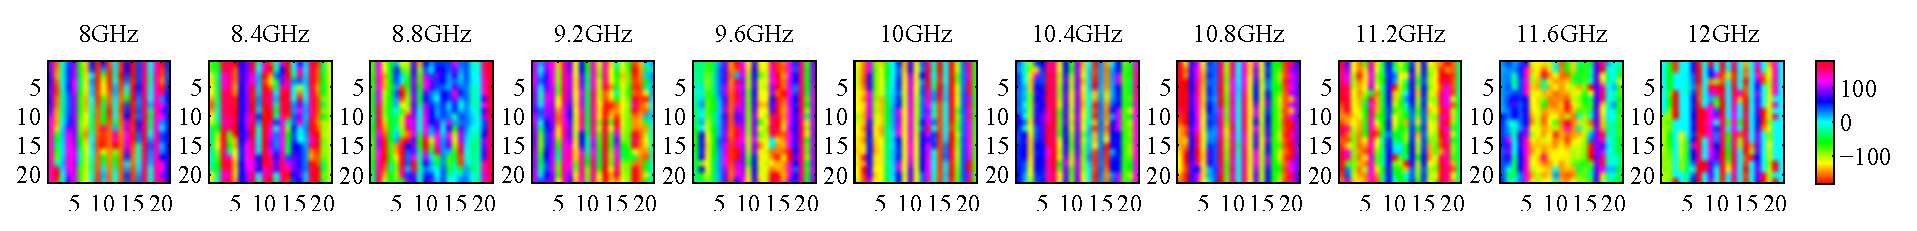
\includegraphics[width =\hsize ]{20150204_mine2_raw_p.eps}
\centering\textmd{data2,位相}
  \end{minipage}
\end{center}
\end{figure}
\begin{figure}[bhtp]
 \begin{center}
     \begin{minipage}[c]{\hsize}
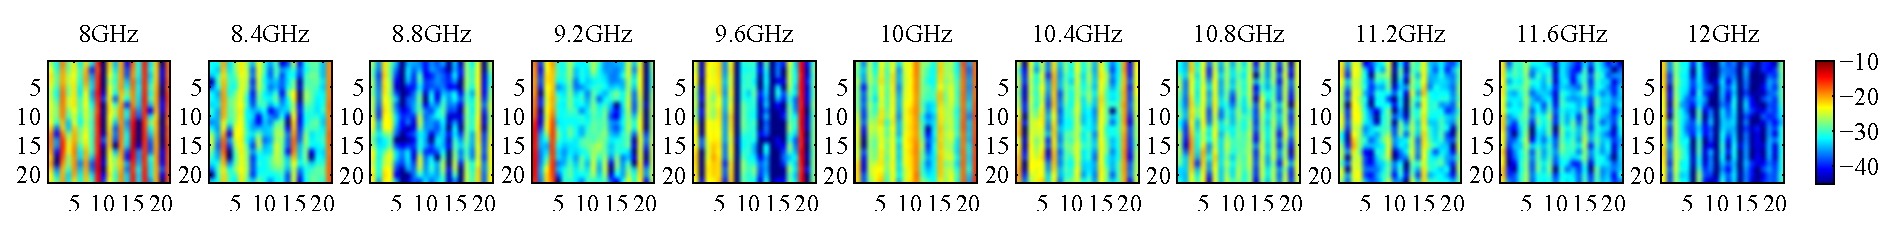
\includegraphics[width = \hsize ]{20150204_mine3_raw_a.eps}
\centering\textmd{data3,振幅}
  \end{minipage}
\\
     \begin{minipage}[c]{\hsize}
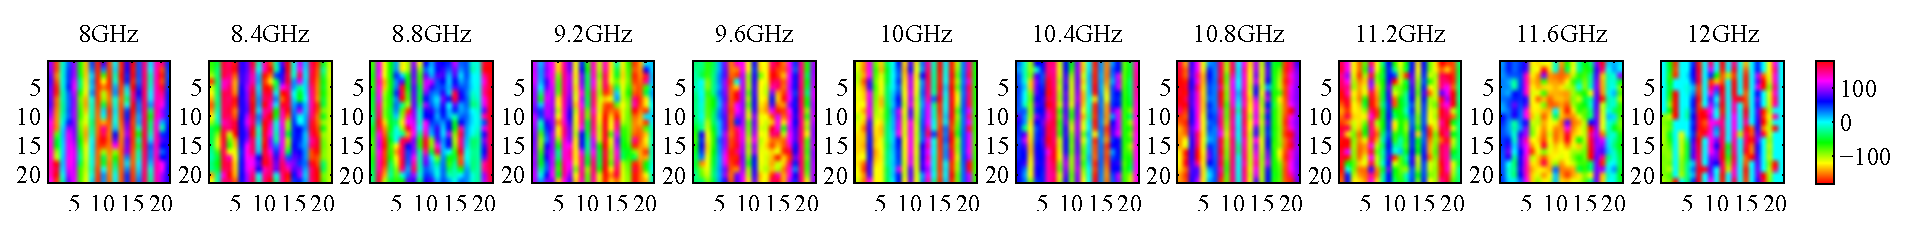
\includegraphics[width =\hsize ]{20150204_mine3_raw_p.eps}
\centering\textmd{data3,位相}
  \end{minipage}
\end{center}
\end{figure}
\begin{figure}[bhtp]
 \begin{center}
     \begin{minipage}[c]{\hsize}
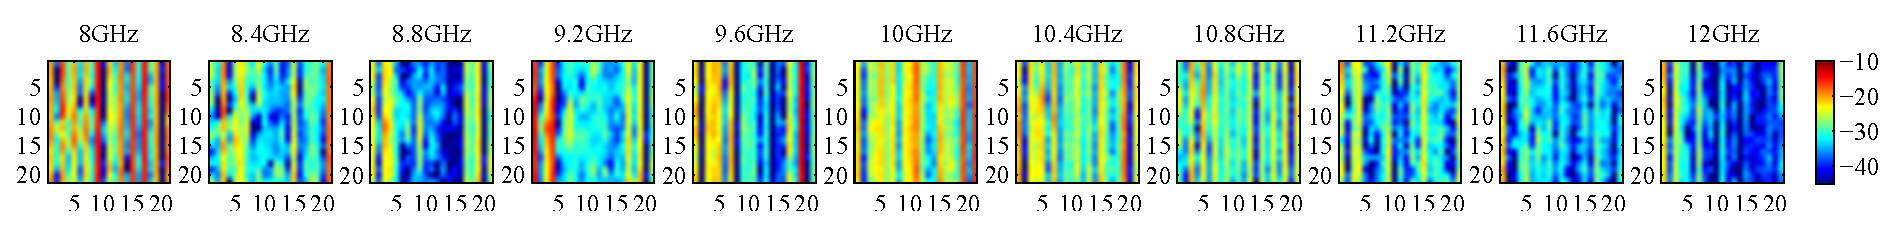
\includegraphics[width = \hsize ]{20150204_mine4_raw_a.eps}
\centering\textmd{data4,振幅}
  \end{minipage}
\\
     \begin{minipage}[c]{\hsize}
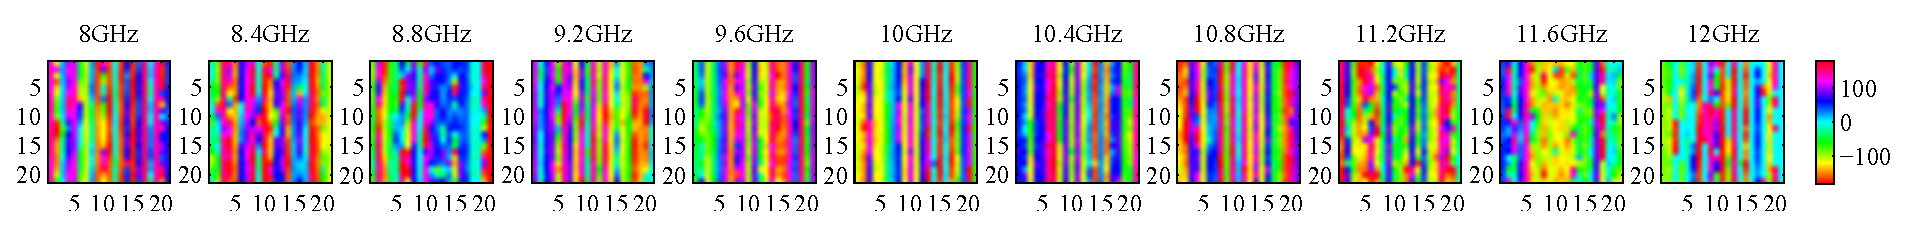
\includegraphics[width =\hsize ]{20150204_mine4_raw_p.eps}
\centering\textmd{data4,位相}
  \end{minipage}
\end{center}
\end{figure}
\begin{figure}[bhtp]
 \begin{center}
     \begin{minipage}[c]{\hsize}
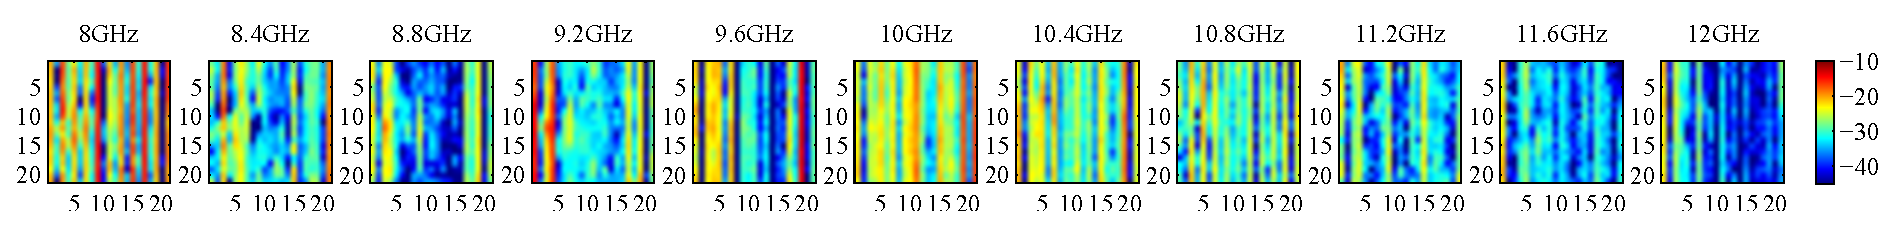
\includegraphics[width = \hsize ]{20150204_mine5_raw_a.eps}
\centering\textmd{data5,振幅}
  \end{minipage}
\\
     \begin{minipage}[c]{\hsize}
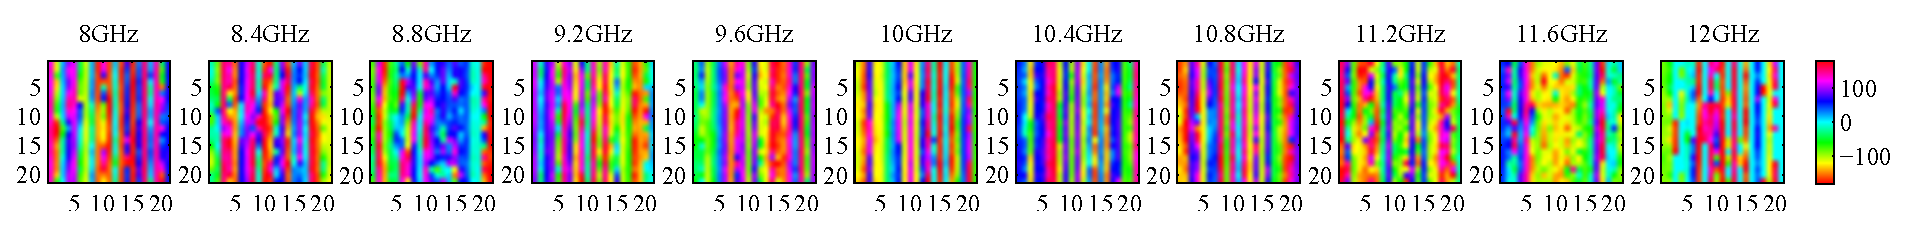
\includegraphics[width =\hsize ]{20150204_mine5_raw_p.eps}
\centering\textmd{data5,位相}
  \end{minipage}
\end{center}
\end{figure}
\begin{figure}[hbtp]
 \begin{center}
     \begin{minipage}[c]{\hsize}
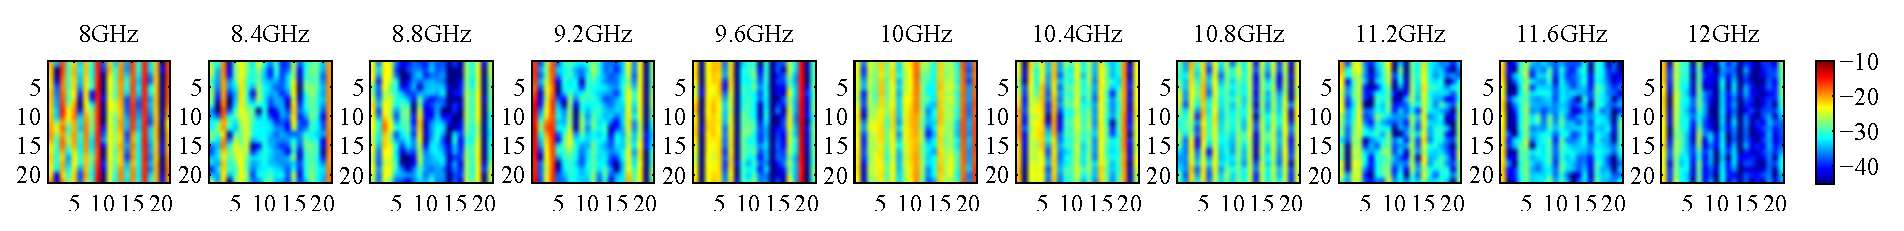
\includegraphics[width = \hsize ]{20150204_mine6_raw_a.eps}
\centering\textmd{data6,振幅}
  \end{minipage}
\\
     \begin{minipage}[c]{\hsize}
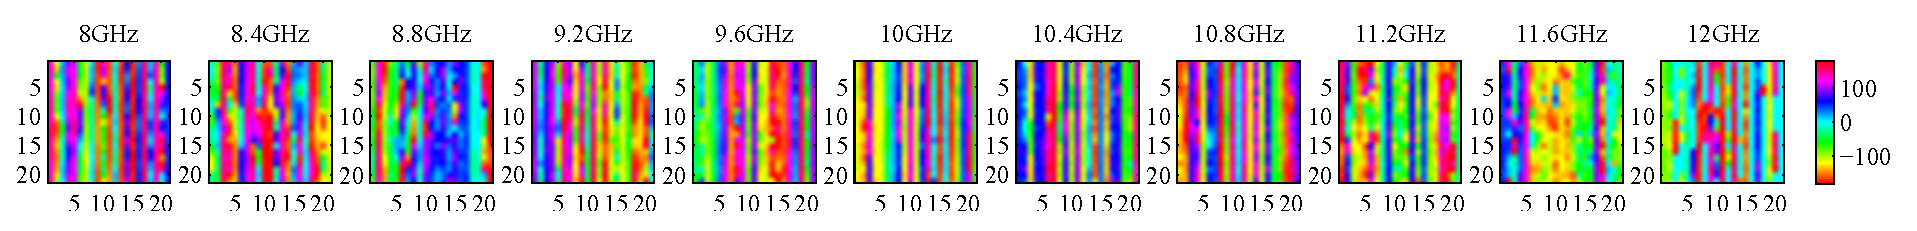
\includegraphics[width =\hsize ]{20150204_mine6_raw_p.eps}
\centering\textmd{data6,位相}
  \end{minipage}
\end{center}
\end{figure}
\begin{figure}[hbtp]
 \begin{center}
     \begin{minipage}[c]{\hsize}
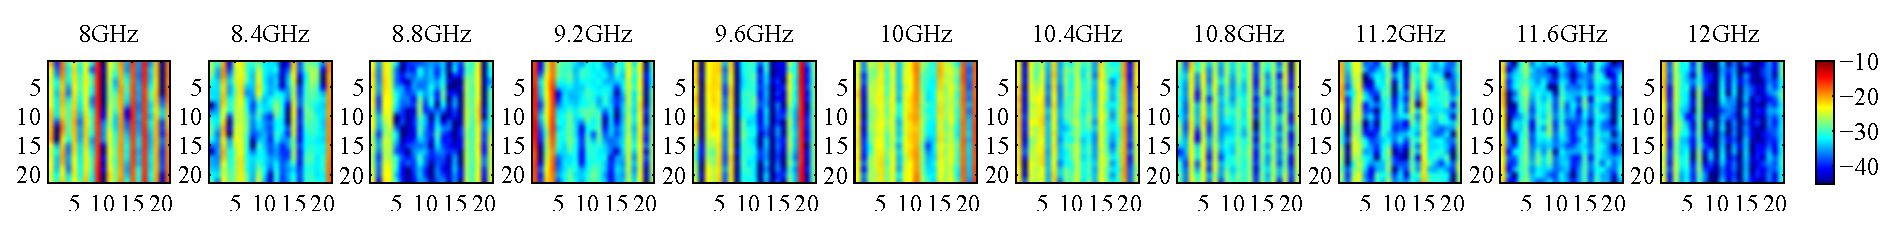
\includegraphics[width = \hsize ]{20150204_mine7_raw_a.eps}
\centering\textmd{data7,振幅}
  \end{minipage}
\\
     \begin{minipage}[c]{\hsize}
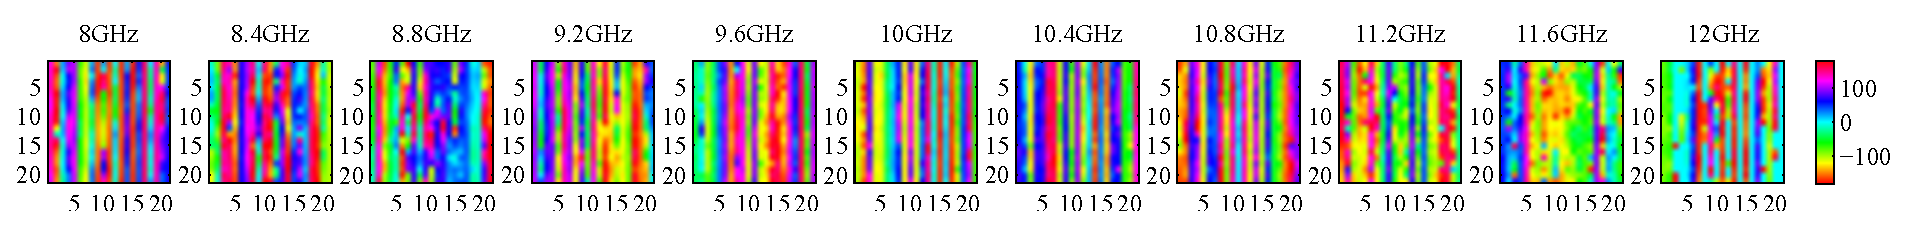
\includegraphics[width =\hsize ]{20150204_mine7_raw_p.eps}
\centering\textmd{data7,位相}
  \end{minipage}
\end{center}
\end{figure}
\begin{figure}[hbtp]
 \begin{center}
     \begin{minipage}[c]{\hsize}
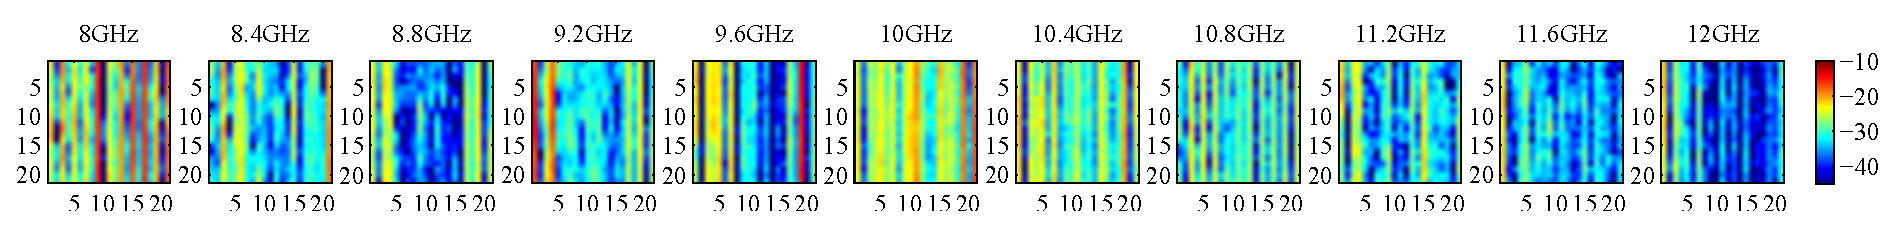
\includegraphics[width = \hsize ]{20150204_mine8_raw_a.eps}
\centering\textmd{data8,振幅}
  \end{minipage}
\\
     \begin{minipage}[c]{\hsize}
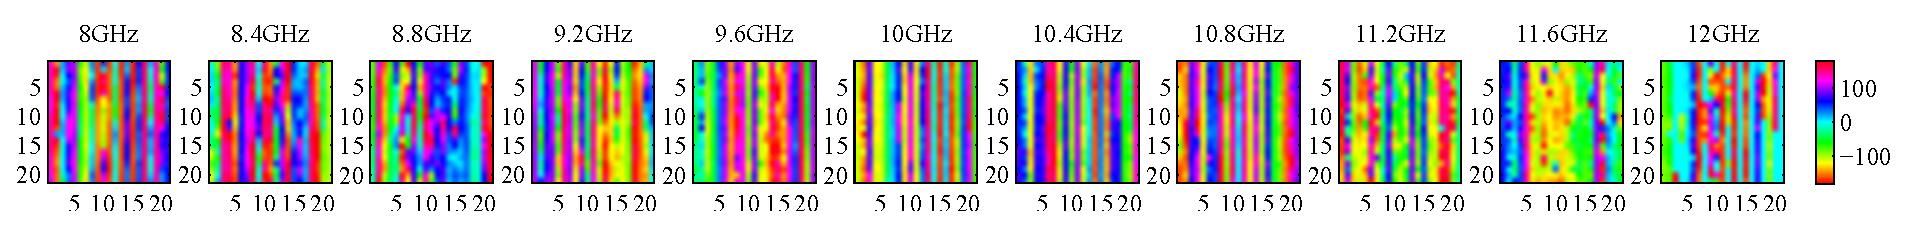
\includegraphics[width =\hsize ]{20150204_mine8_raw_p.eps}
\centering\textmd{data8,位相}
  \end{minipage}
\end{center}
\end{figure}
\begin{figure}[hbtp]
 \begin{center}
     \begin{minipage}[c]{\hsize}
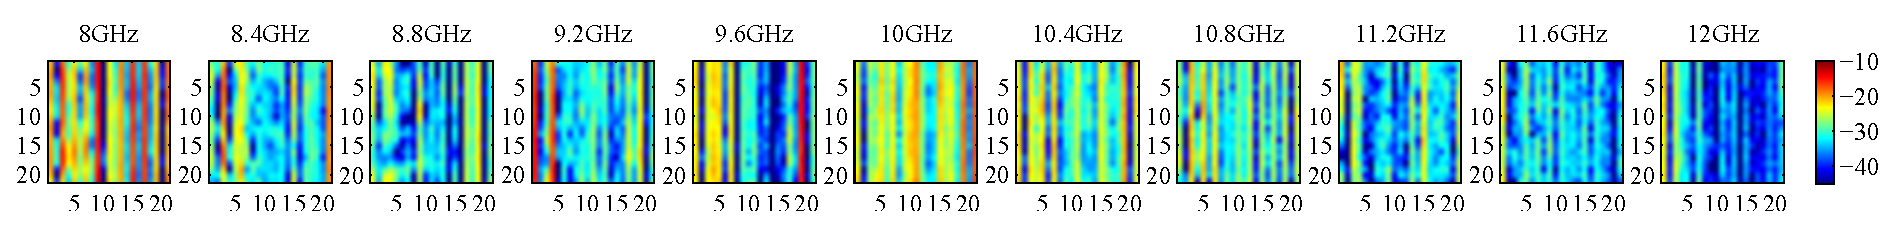
\includegraphics[width = \hsize ]{20150204_mine9_raw_a.eps}
\centering\textmd{data9,振幅}
  \end{minipage}
\\
     \begin{minipage}[c]{\hsize}
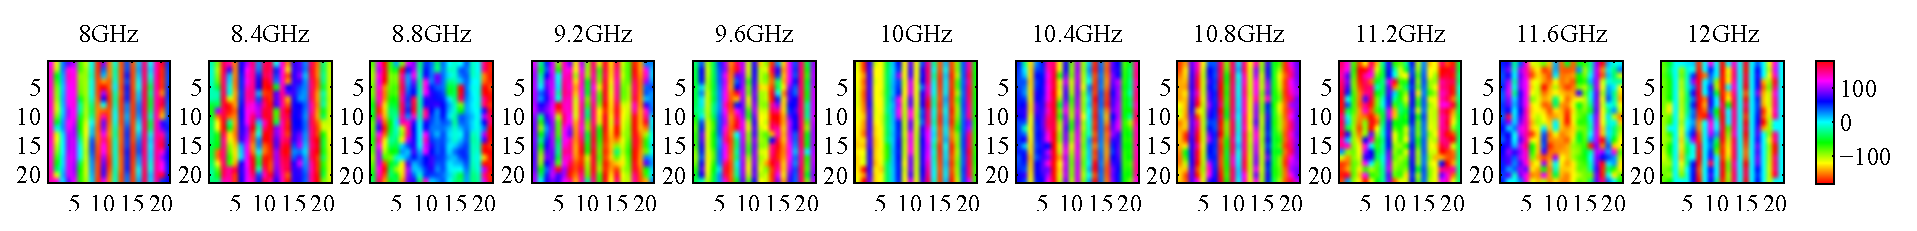
\includegraphics[width =\hsize ]{20150204_mine9_raw_p.eps}
\centering\textmd{data9,位相}
  \end{minipage}
\end{center}
\end{figure}
\begin{figure}[hbtp]
 \begin{center}
     \begin{minipage}[c]{\hsize}
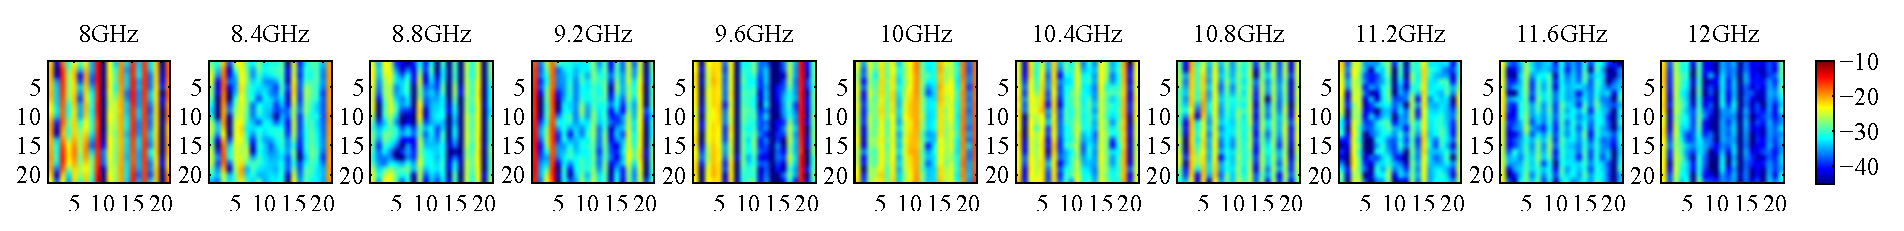
\includegraphics[width = \hsize ]{20150204_mine10_raw_a.eps}
\centering\textmd{data10,振幅}
  \end{minipage}
\\
     \begin{minipage}[c]{\hsize}
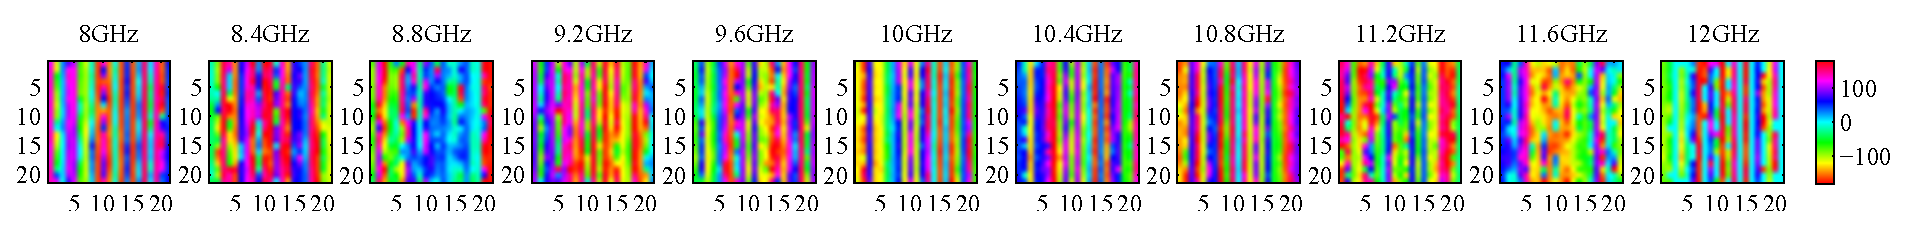
\includegraphics[width =\hsize ]{20150204_mine10_raw_p.eps}
\centering\textmd{data10,位相}
  \end{minipage}
\\
\caption{模擬地雷を埋設して計測したデータ}
\label{mine-raw}
 \end{center}
\end{figure}
\begin{figure}[hbtp]
 \begin{center}
     \begin{minipage}[c]{\hsize}
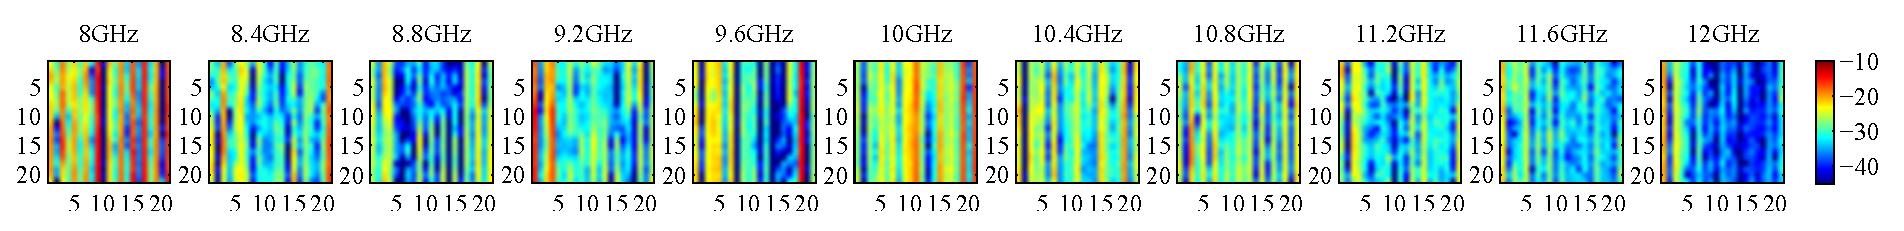
\includegraphics[width = \hsize ]{20150204_none1_raw_a.eps}
\centering\textmd{振幅}
  \end{minipage}
\\
     \begin{minipage}[c]{\hsize}
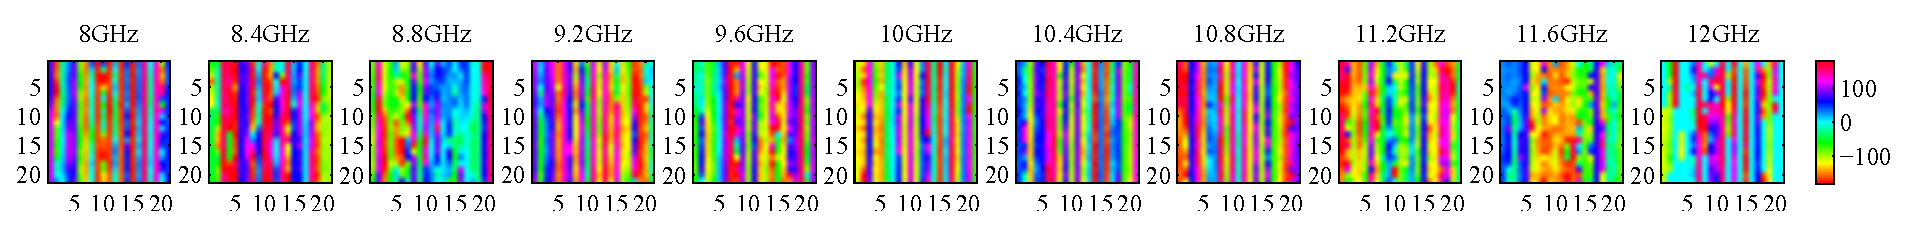
\includegraphics[width =\hsize ]{20150204_none1_raw_p.eps}
\centering\textmd{位相}
  \end{minipage}
\caption{模擬地雷のない地面を計測したデータ}
\label{none-raw} 
 \end{center}
\end{figure}
\begin{figure}[hbtp]
 \begin{center}
     \begin{minipage}[c]{\hsize}
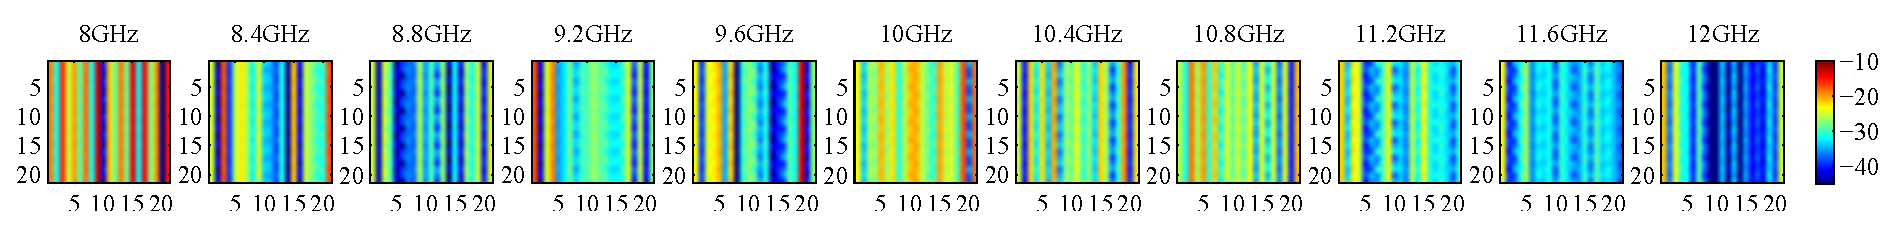
\includegraphics[width = \hsize ]{20150206_direct2_raw_a.eps}
\centering\textmd{振幅}
  \end{minipage}
\\
     \begin{minipage}[c]{\hsize}
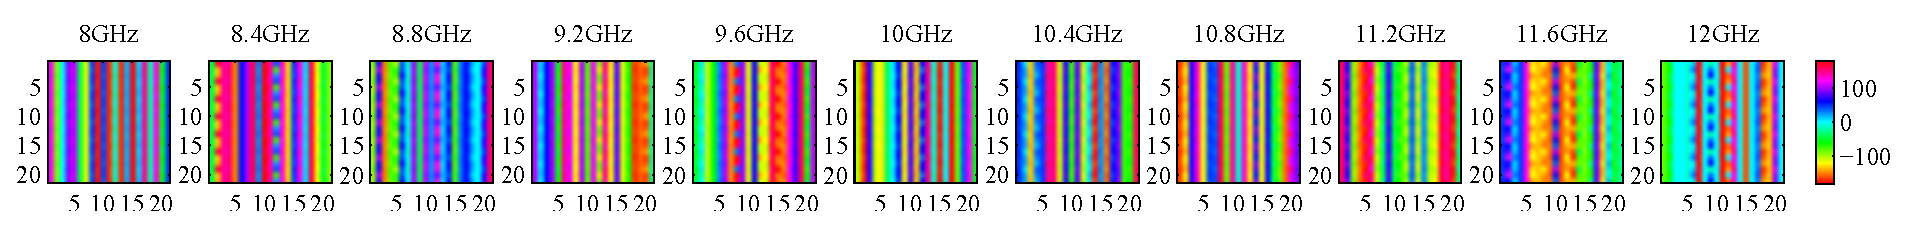
\includegraphics[width =\hsize ]{20150206_direct2_raw_p.eps}
\centering\textmd{位相}
  \end{minipage}
\caption{空中を計測したデータ}
\label{direct-raw}
 \end{center}
\end{figure}
\begin{figure}[hbtp]
 \begin{center}
     \begin{minipage}[c]{\hsize}
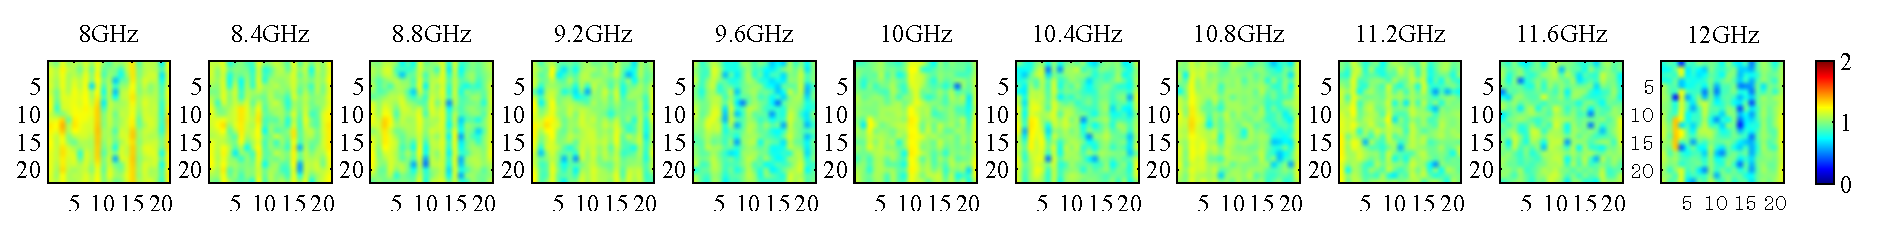
\includegraphics[width = \hsize ]{20150204_mine6_Bhosei_a.eps}
\centering\textmd{振幅}
  \end{minipage}
\\
     \begin{minipage}[c]{\hsize}
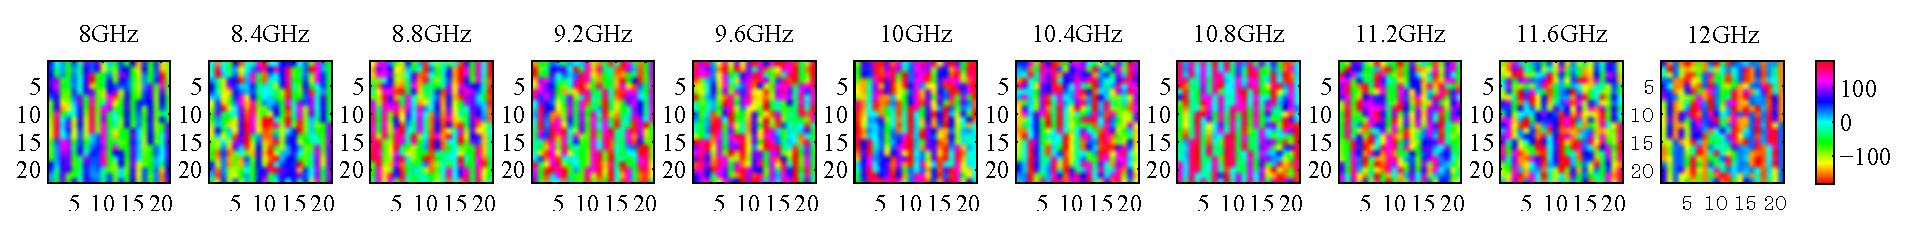
\includegraphics[width =\hsize ]{20150204_mine6_Bhosei_p.eps}
\centering\textmd{位相}
  \end{minipage}
\caption{data6を補正した後の画像}
\label{mine6-hosei}
 \end{center}
\end{figure}
\newpage
\chapter{提案1: アンテナ素子のエレメント外周の曲線化}
\section{Taper-Walled LTSAをアレイ化した際の問題点}
以前われわれが提案したTaper-Walled LTSAを使用することを検討した.
このLTSAは図\ref{pic:twltsa}のように壁面をTaper状に加工することで,同じく以前に
本研究室が提案したWalled LTSAよりも図\ref{pic:twltsa-dc}のように更に直接結合を軽減することが
できる\cite{2011Nakano}.

\begin{figure}[t]
\begin{center}
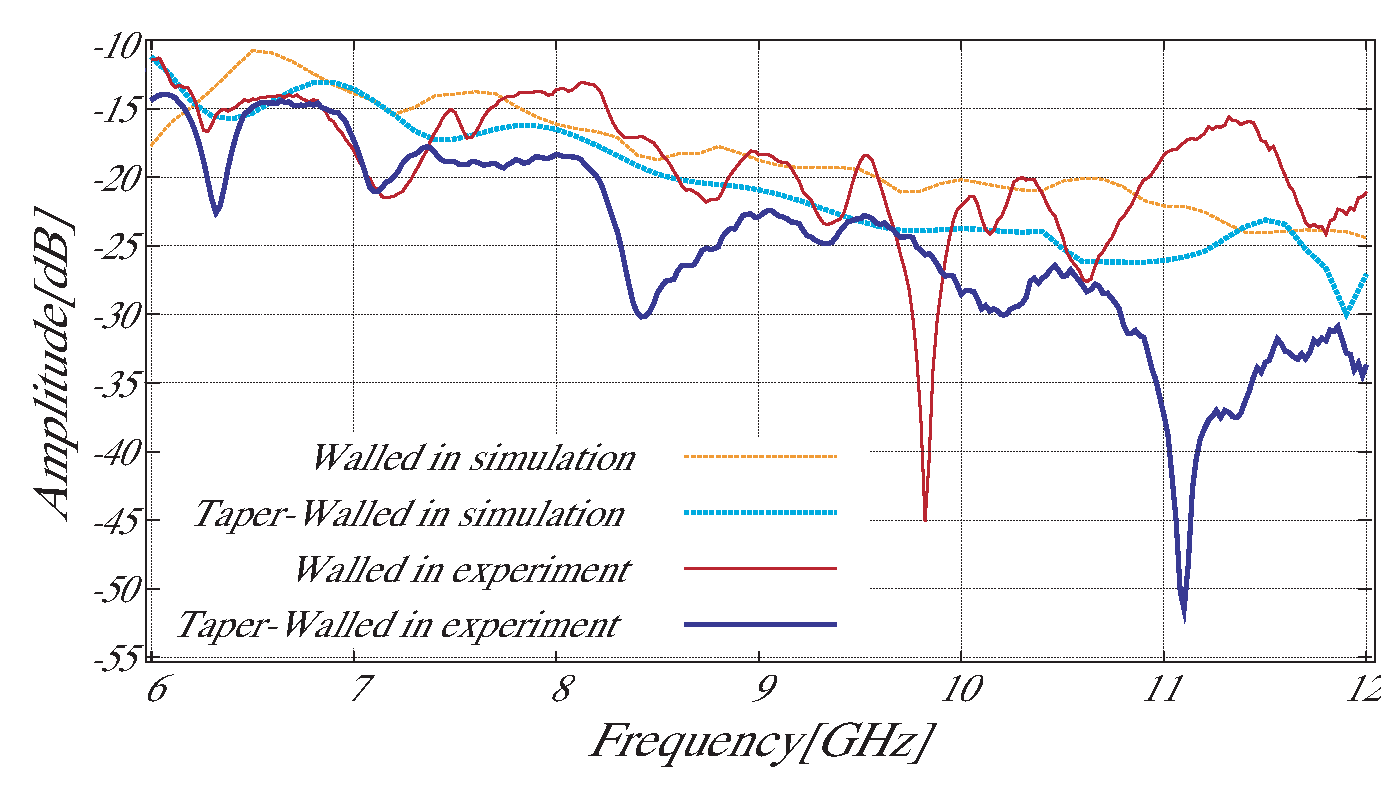
\includegraphics[width =\hsize]{walled-twalled.eps}
\caption{Walled LTSAとTaper-Walled LTSAの直接結合\cite{2011Nakano}} \label{pic:twltsa-dc} 
\end{center}
\end{figure}

まず,同様のアンテナエレメントを12個並べた図\ref{pic:array}のアレイアンテナで
反射特性と直接結合を計測した.しかし,
エレメントの個体差が大きく出てしまった.図\ref{old-solo-S11}
,図\ref{old-solo-S21}に示すのは,特に反射特性の悪かった
エレメントの反射特性と直接結合である.
これは主にアルミで形成された導波管のひずみによるものと考えられる.
特に,反射特性においては図\ref{old-solo-S11}のように
アンテナとして実用的に下回るべきとされるラインの
--10dBを超えてしまっているものもあった.

そこで,Taper-Walled LTSAのエレメント(図\ref{TWLTSA})に着目し,
エレメントの外周を曲線的にし,反射特性を低減させた図\ref{curved}のアンテナを
製作した.
このアンテナの反射特性と直接結合を計測したところ,図\ref{new-solo-S11},\ref{new-solo-S21}
のようになり,反射特性は向上し,直接結合においてもTaper-Walled LTSA
に遜色ない結果になった.

\begin{figure}[t]
\begin{center}
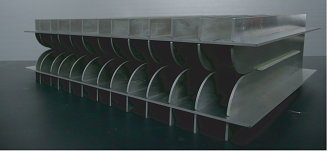
\includegraphics[width =\hsize]{array_antenna.png}
\caption{製作した一次元アレイアンテナ} \label{pic:array} 
\end{center}
\end{figure}

\begin{figure}[t]
\begin{center}
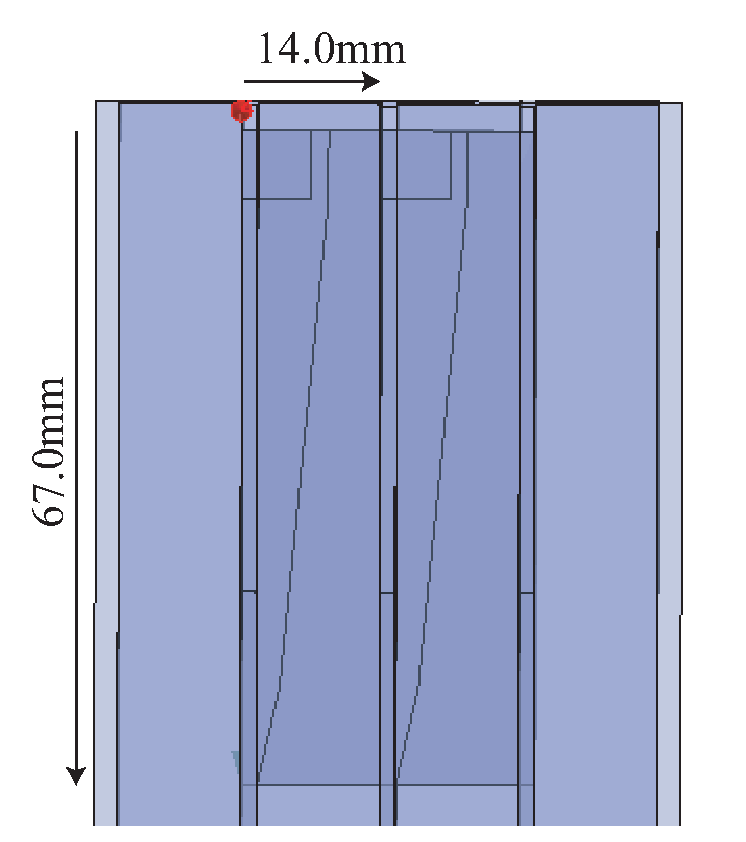
\includegraphics[width =\hsize]{TWLTSA.eps}
\caption{Taper-Walled LTSAのエレメント} \label{TWLTSA} 
\end{center}
\end{figure}

\begin{figure}[t]
\begin{center}
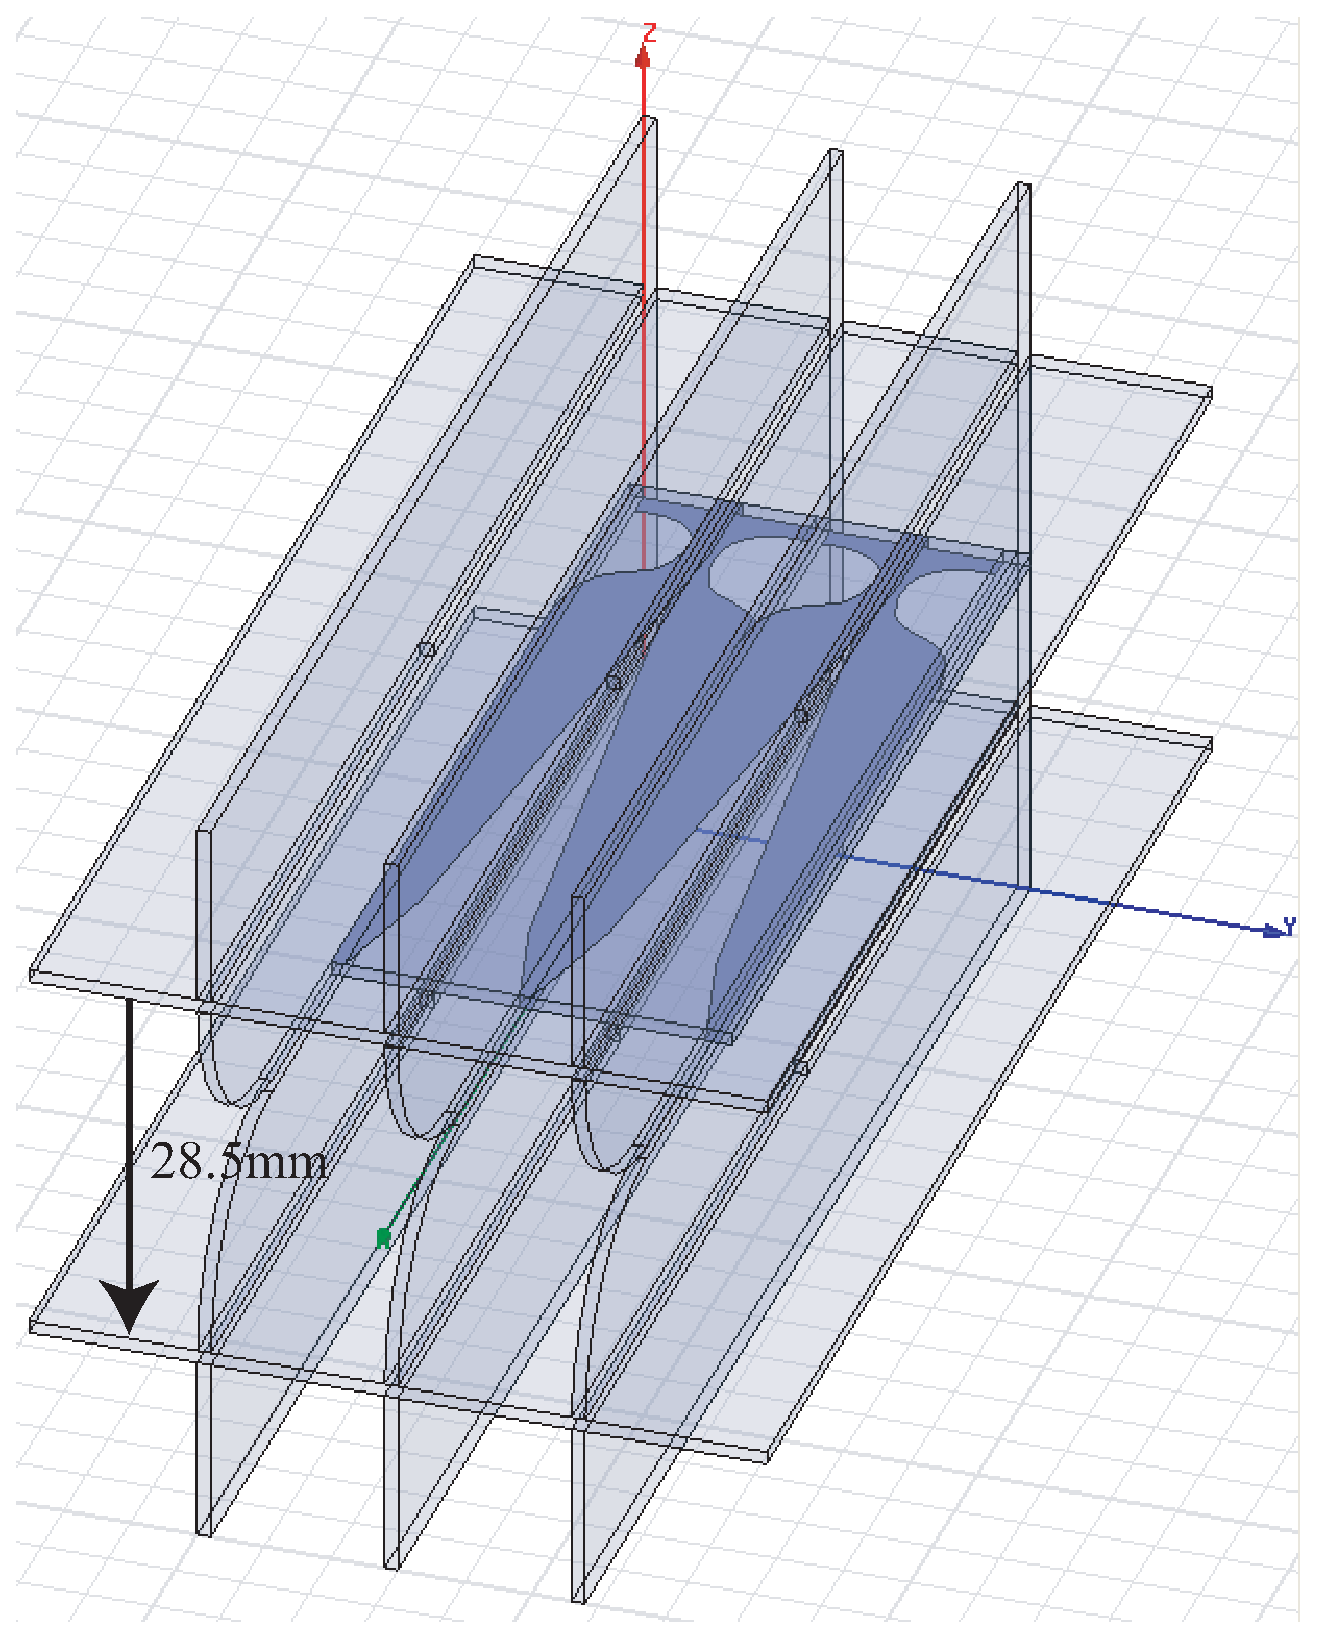
\includegraphics[width =\hsize]{curvedantenna2.eps}
\caption{外周が曲線のTaper-Walled LTSA} \label{curved} 
\end{center}
\end{figure}

\begin{figure}[t]
\begin{center}
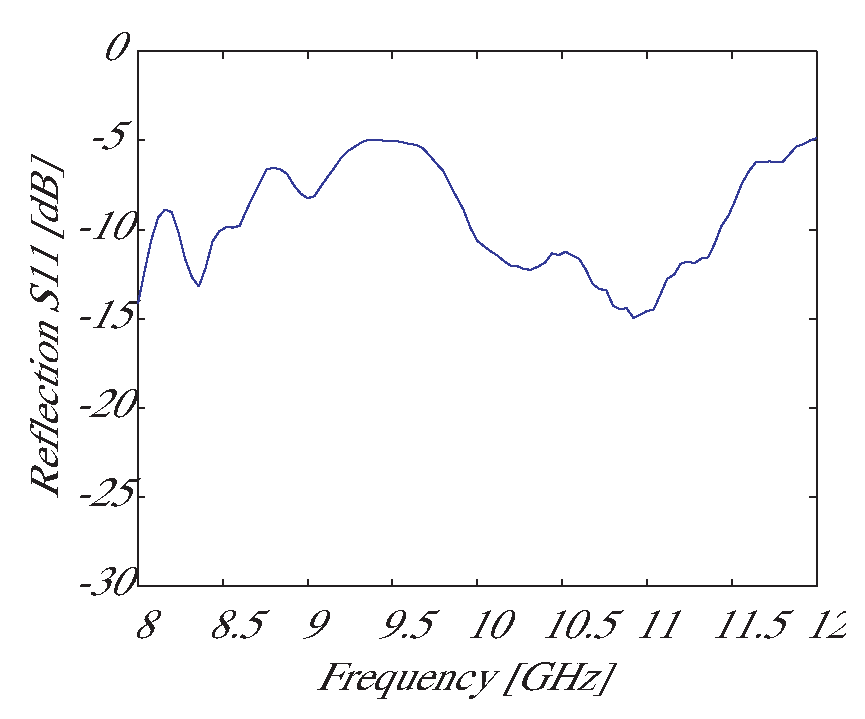
\includegraphics[width =\hsize]{oldantenna_S11.eps}
\caption{外周が曲線のTaper-Walled LTSAの反射特性}
\label{old-solo-S11}
\end{center}
\end{figure}

\begin{figure}[t]
\begin{center}
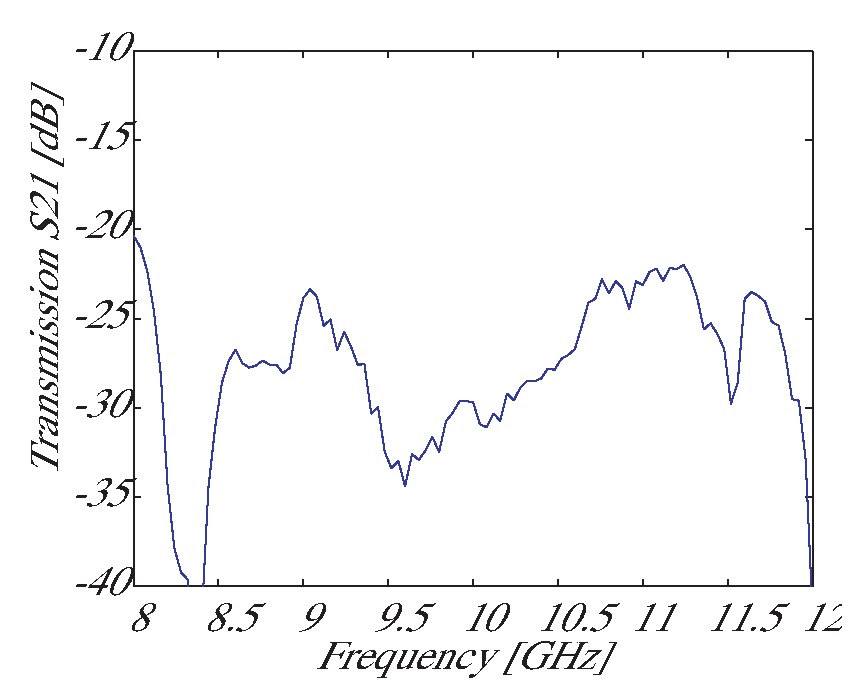
\includegraphics[width =\hsize]{oldantenna_S21.eps}
\caption{外周が曲線のTaper-Walled LTSAの直接結合}
\label{old-solo-S21}
\end{center}
\end{figure}

\begin{figure}[t]
\begin{center}
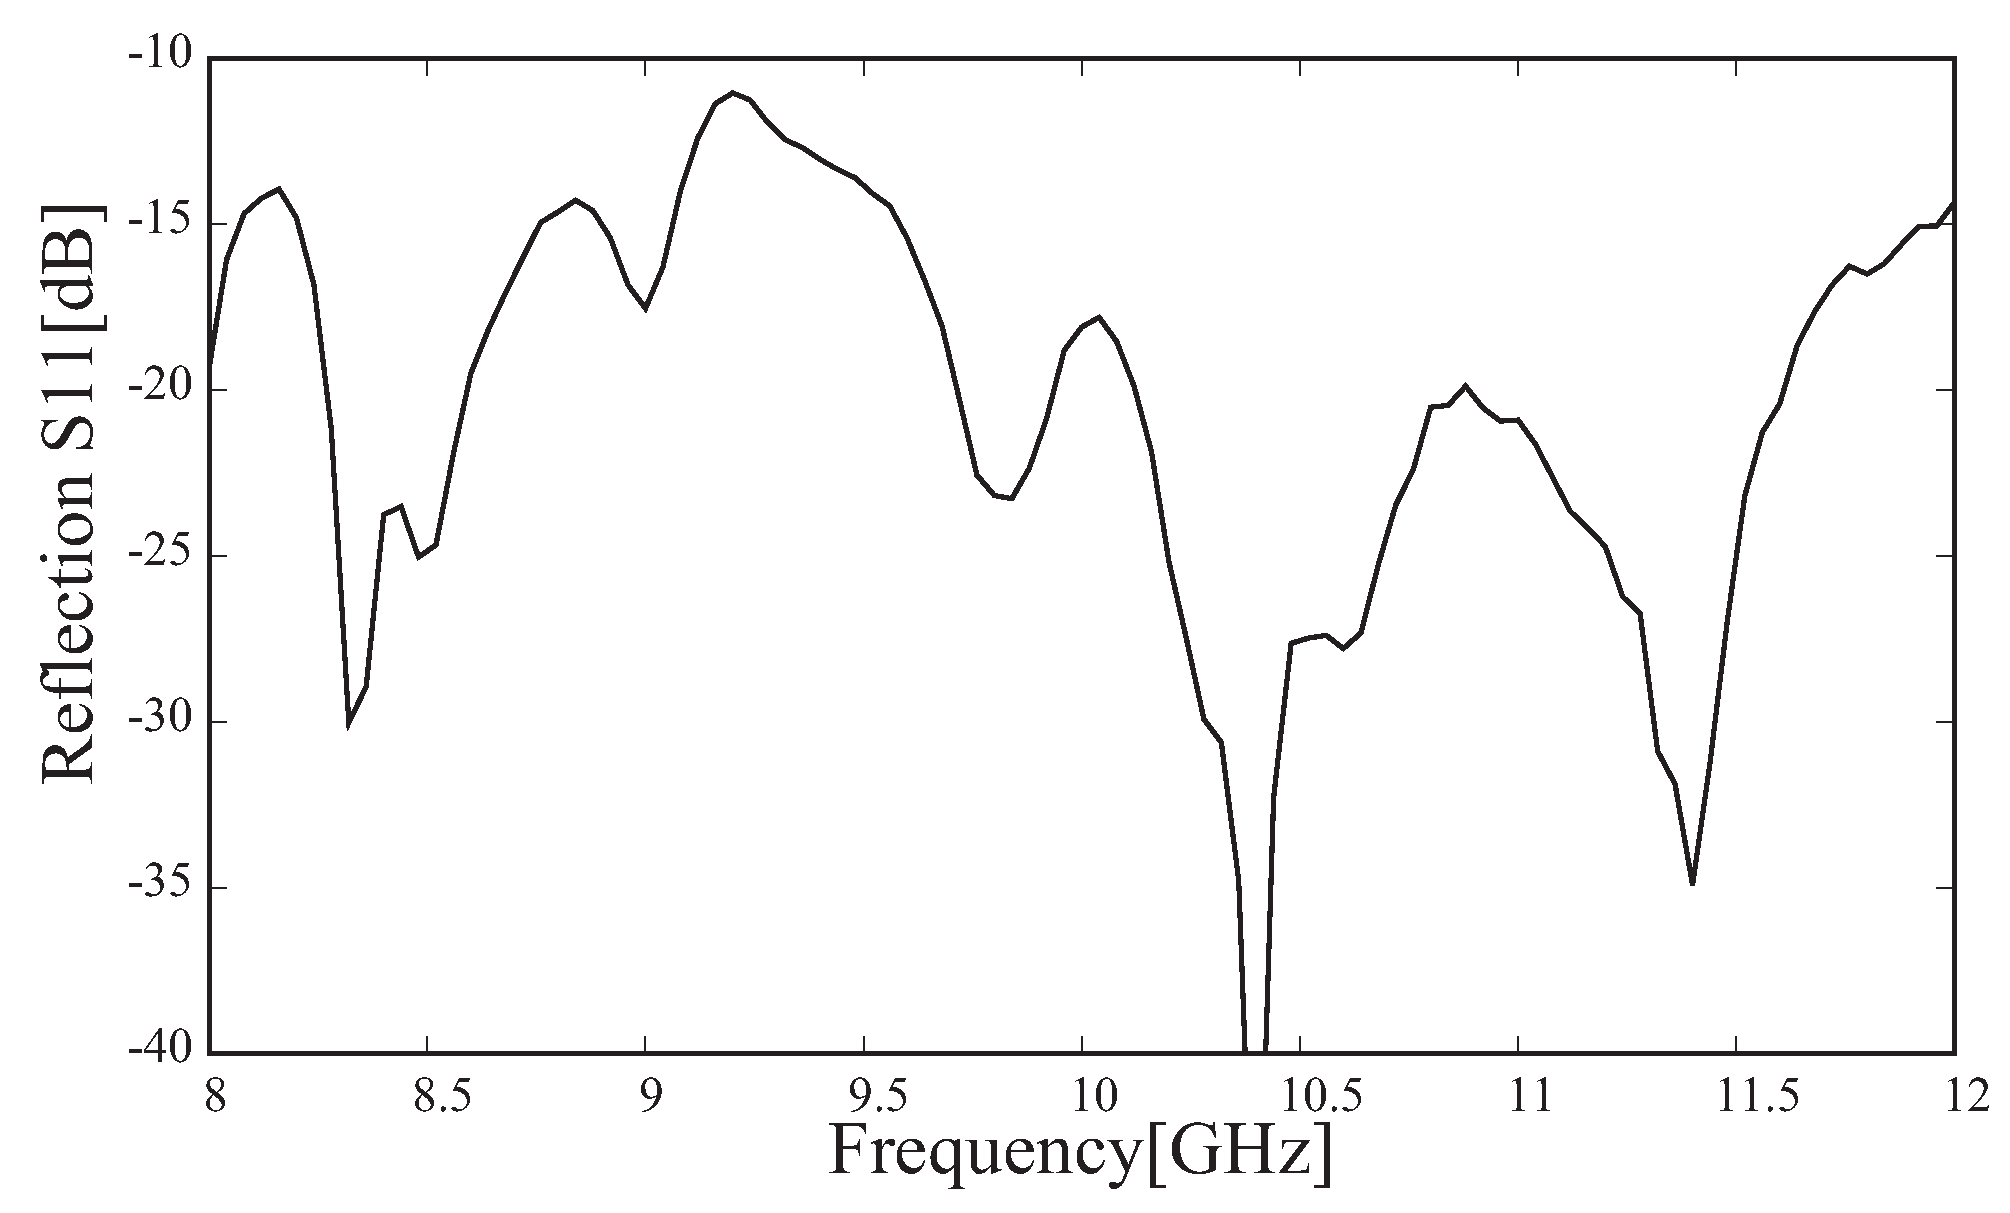
\includegraphics[width =\hsize]{new_solo_S11.eps}
\caption{外周が曲線のTaper-Walled LTSAの反射特性}
\label{new-solo-S11}
\end{center}
\end{figure}

\begin{figure}[t]
\begin{center}
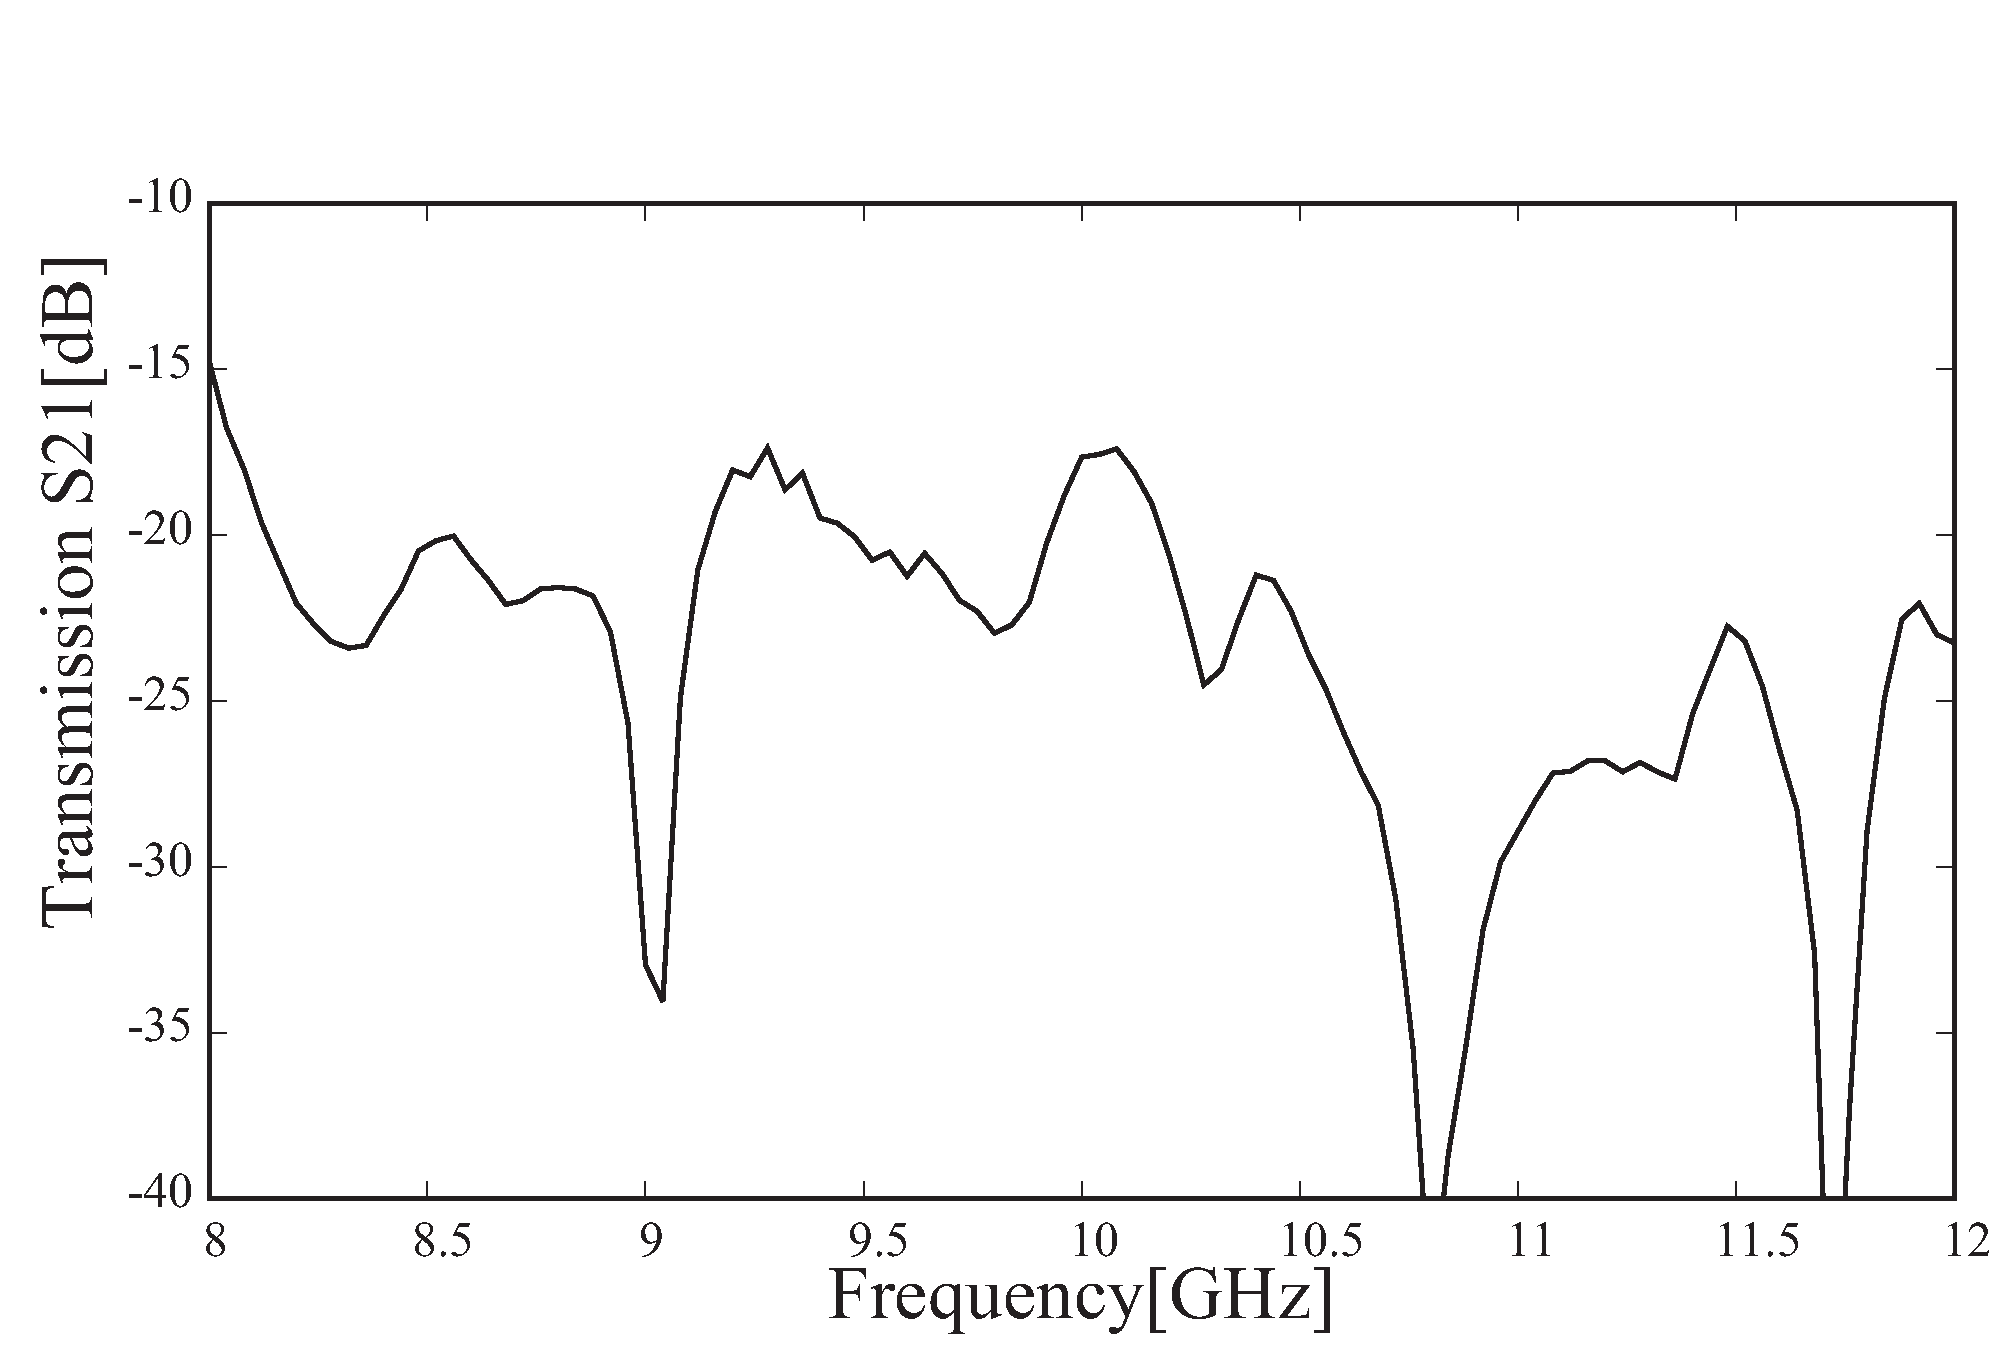
\includegraphics[width =\hsize]{new_solo_S21_dc.eps}
\caption{外周が曲線のTaper-Walled LTSAの直接結合}
\label{new-solo-S21}
\end{center}
\end{figure}

\section{新型フロントエンドのアレイアンテナとしての評価}
\begin{figure}[t]
\begin{center}
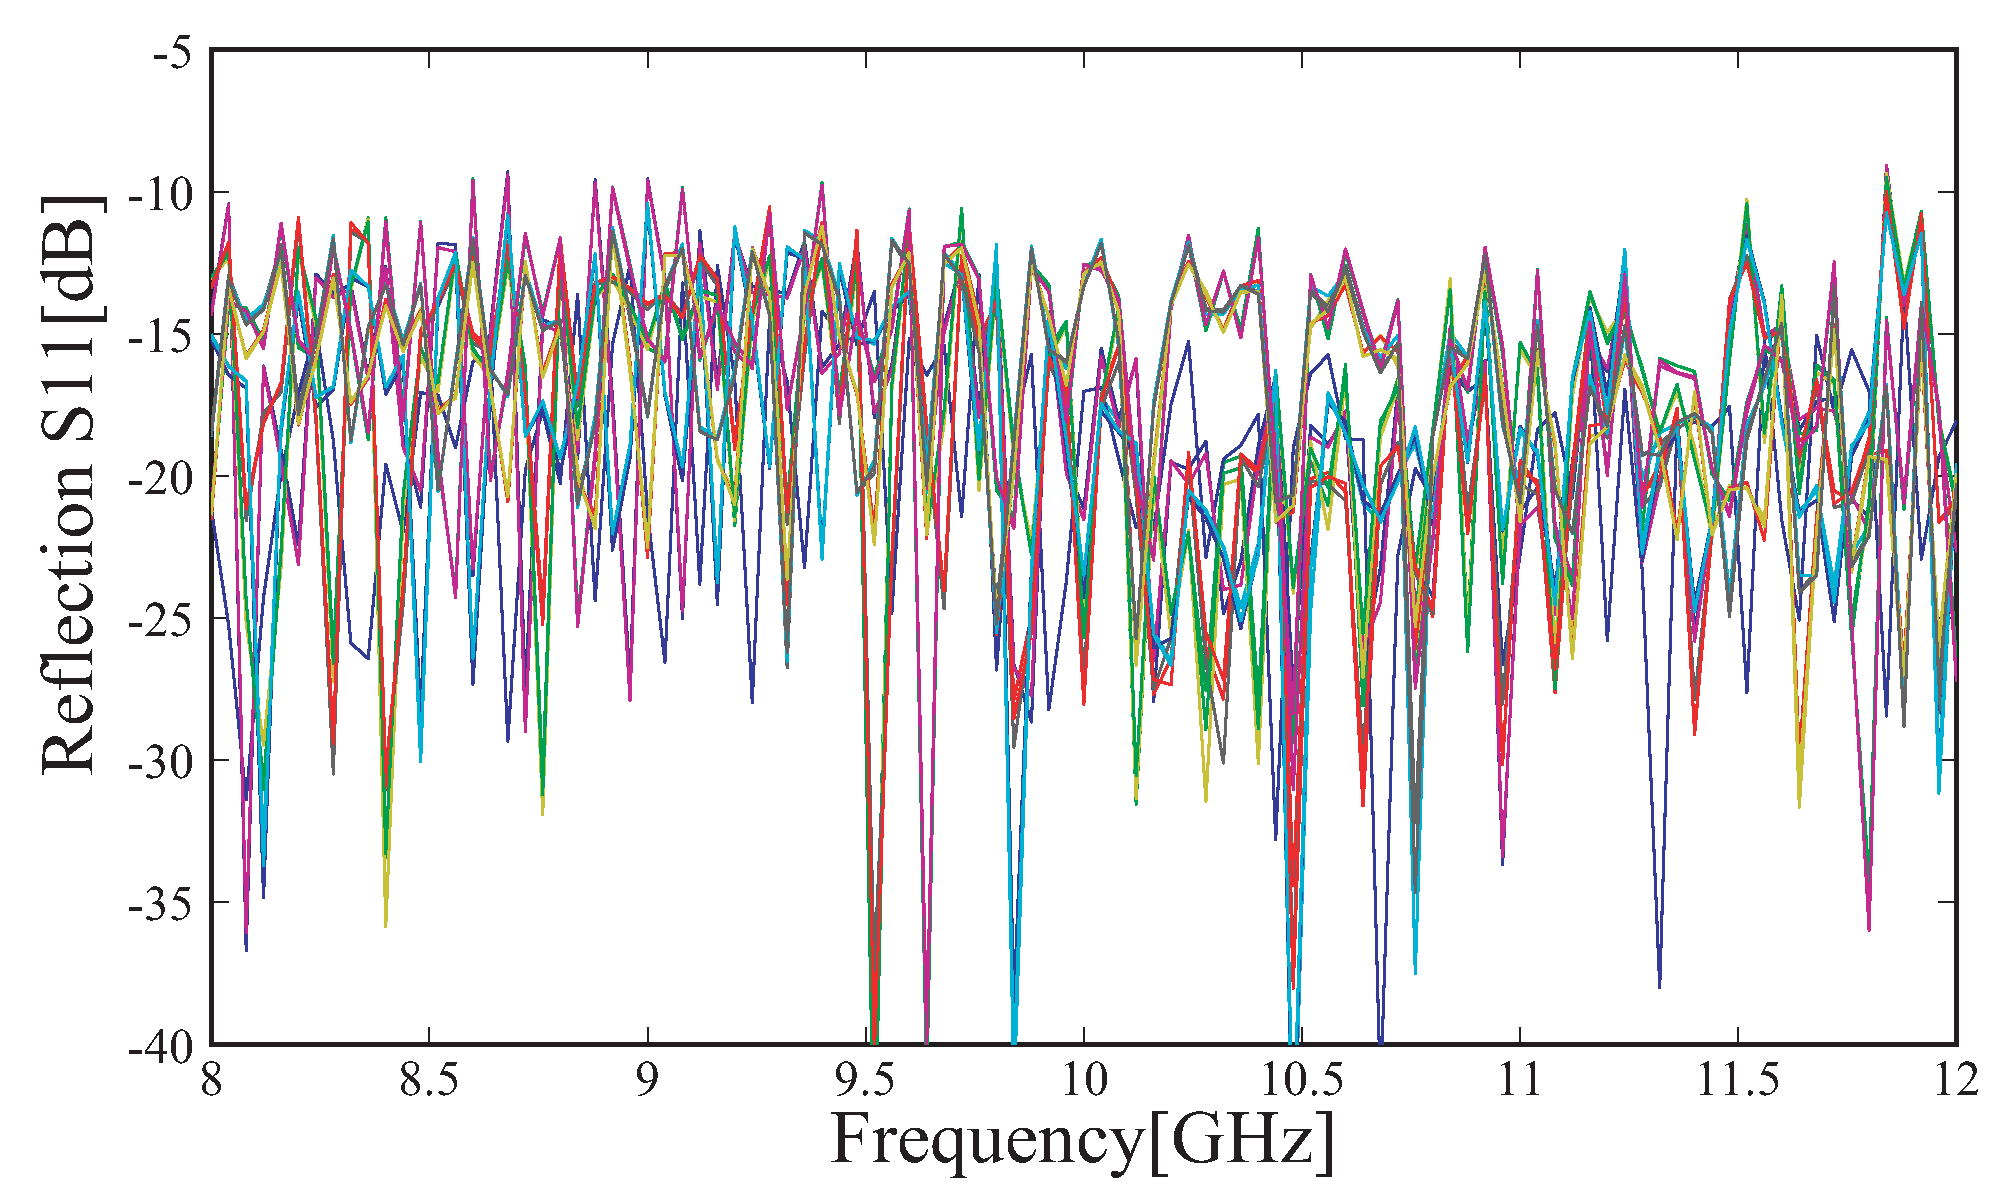
\includegraphics[width =\hsize]{old_S11.eps}
\caption{Taper-Walled LTSAのアレイ化した反射特性} \label{pic:twltsa-1} 
\end{center}
\end{figure}

\begin{figure}[t]
\begin{center}
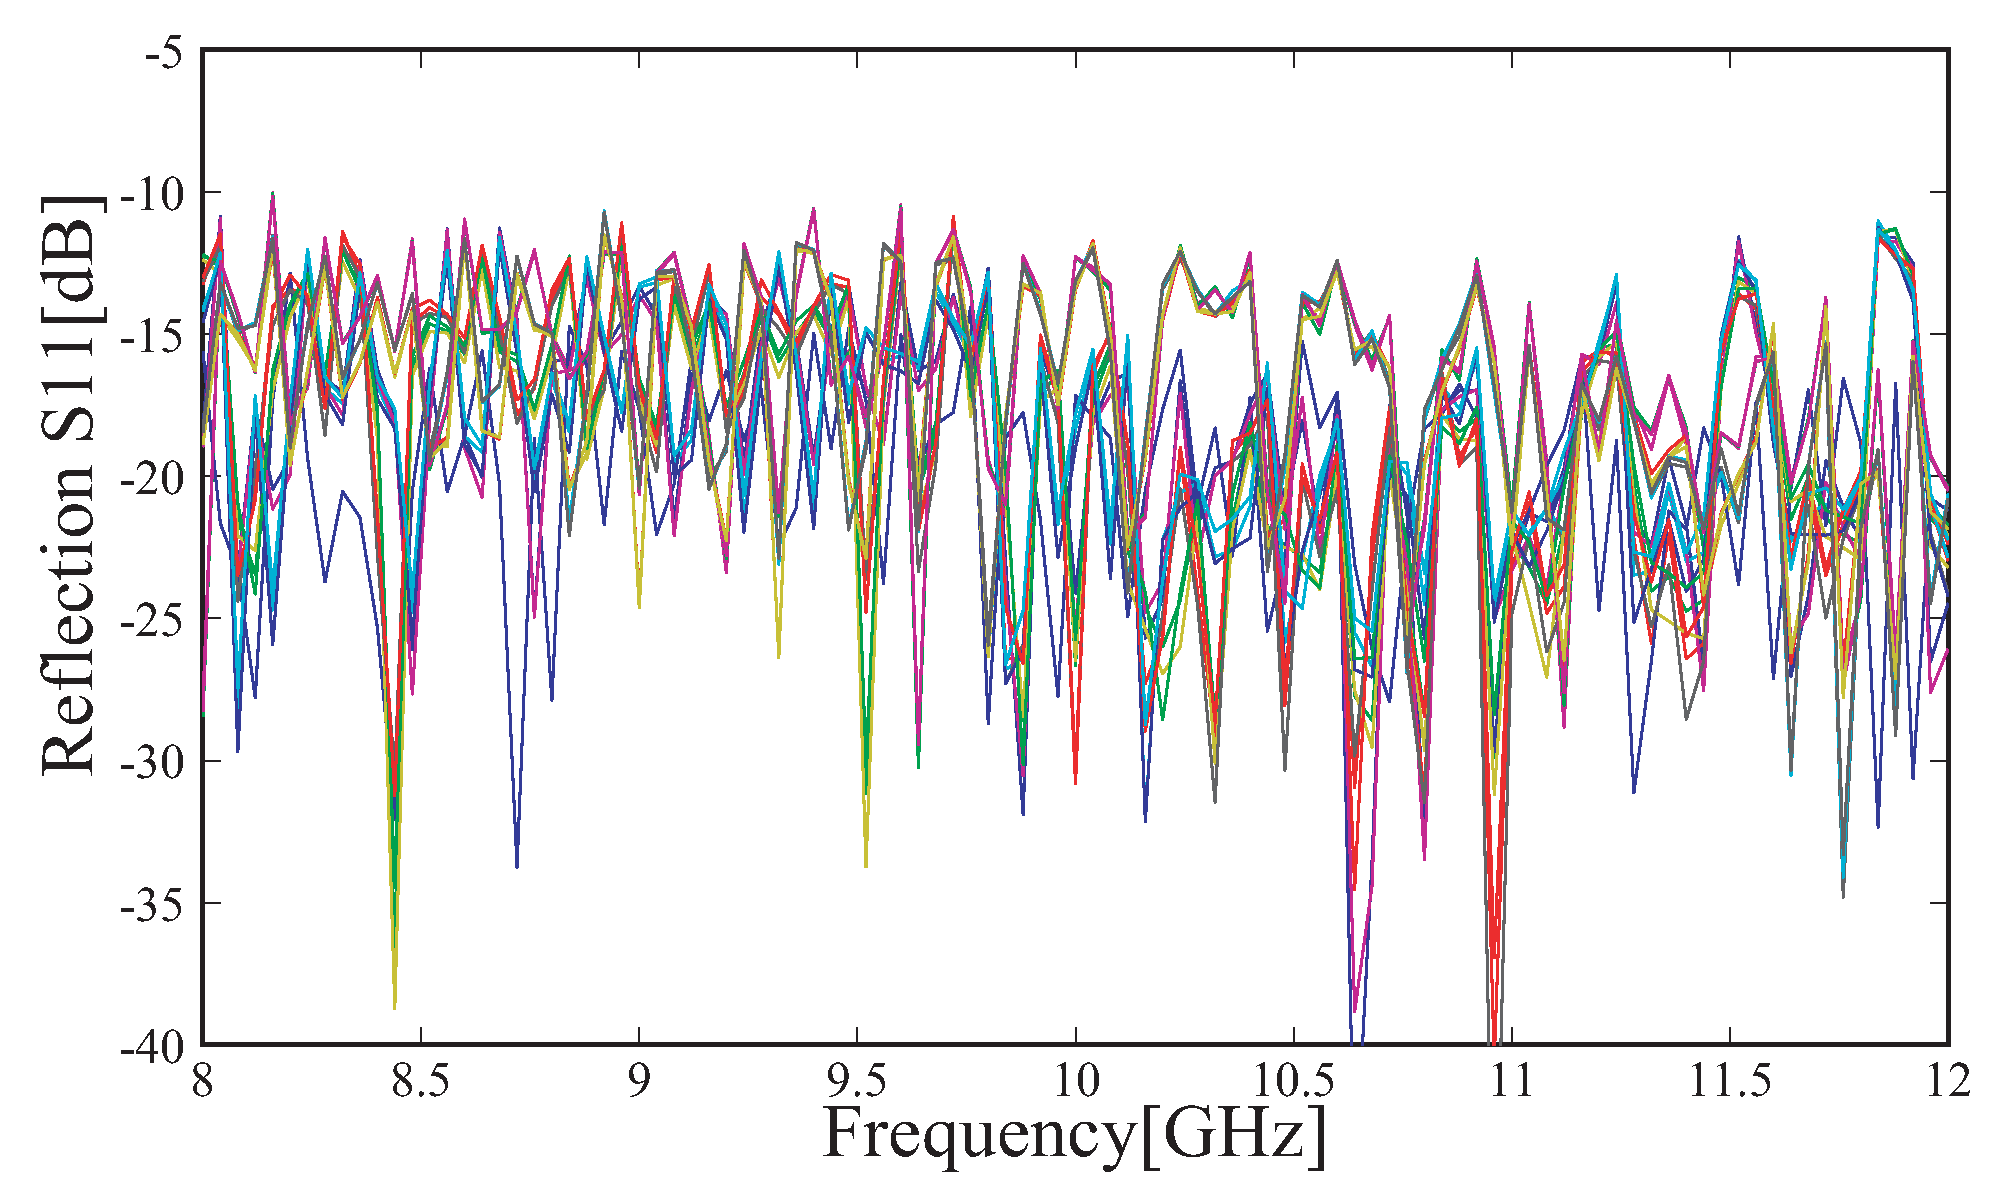
\includegraphics[width =\hsize]{new_S11.eps}
\caption{外周が曲線のTaper-Walled LTSAのアレイ化した反射特性}
\label{pic:ctwltsa-1} 
\end{center}
\end{figure}

\begin{figure}[t]
\begin{center}
\includegraphics[width =\hsize]{old_S21_dc_e.eps}
\caption{Taper-Walled LTSAのアレイ化した直接結合} \label{pic:twltsa-2} 
\end{center}
\end{figure}

\begin{figure}[t]
\begin{center}
\includegraphics[width =\hsize]{new_S21_dc_e.eps}
\caption{外周が曲線のTaper-Walled LTSAのアレイ化した直接結合}
\label{pic:ctwltsa-2} 
\end{center}
\end{figure}
\section{フロントエンドに実装しての比較}
Taper-Walled LTSAのアレイ化しスイッチ部を含めたフロントエンド全体での
反射特性と直接結合は図\ref{pic:twltsa-1},\ref{pic:twltsa-2}のようになった.
外周が曲線のTaper-Walled LTSAについても同様にアレイ化しフロントエンド全体で計測した.
反射特性と直接結合は図\ref{pic:ctwltsa-1},\ref{pic:ctwltsa-2}のようになり,個体差が減少した.
直接結合が約--30dB以下と小さく出ているのは,スイッチ部の減衰によるものと考えられる.
直接結合については,高周波領域において通常のTaper-Walled LTSAよりも大きく出ているが,
図\ref{pic:twltsa-dc}と図\ref{new-solo-S21}を考慮すれば,Walled LTSAよりも低く実用に問題ない範囲と言える.
\clearpage
\section{計測実験}
このフロントエンドを用いて同様の模擬地雷計測実験を行った.結果を
図\ref{mine-ctwltsa}に示す.入力値が全体的に向上し,地雷の形状が
人間の目で見てもより明確になったことが分かる.
\begin{figure}[hbtp]
 \begin{center}
     \begin{minipage}[c]{\hsize}
\includegraphics[width = \hsize ]{20170205_mine1_a.eps}
\centering\textmd{data1,振幅}
  \end{minipage}
\\
     \begin{minipage}[c]{\hsize}
\includegraphics[width = \hsize ]{20170205_mine1_p.eps}
\centering\textmd{data1,位相}
  \end{minipage}
\end{center}
\end{figure}
\begin{figure}[bhtp]
 \begin{center}
     \begin{minipage}[c]{\hsize}
\includegraphics[width = \hsize ]{20170205_mine2_a.eps}
\centering\textmd{data2,振幅}
  \end{minipage}
\\
     \begin{minipage}[c]{\hsize}
\includegraphics[width = \hsize ]{20170205_mine2_p.eps}
\centering\textmd{data2,位相}
  \end{minipage}
\end{center}
\end{figure}
\begin{figure}[bhtp]
 \begin{center}
     \begin{minipage}[c]{\hsize}
\includegraphics[width = \hsize ]{20170205_mine3_a.eps}
\centering\textmd{data3,振幅}
  \end{minipage}
\\
     \begin{minipage}[c]{\hsize}
\includegraphics[width = \hsize ]{20170205_mine3_p.eps}
\centering\textmd{data3,位相}
  \end{minipage}
\end{center}
\end{figure}
\begin{figure}[bhtp]
 \begin{center}
     \begin{minipage}[c]{\hsize}
\includegraphics[width = \hsize ]{20170205_mine4_a.eps}
\centering\textmd{data4,振幅}
  \end{minipage}
\\
     \begin{minipage}[c]{\hsize}
\includegraphics[width = \hsize ]{20170205_mine4_p.eps}
\centering\textmd{data4,位相}
  \end{minipage}
\end{center}
\end{figure}
\begin{figure}[bhtp]
 \begin{center}
     \begin{minipage}[c]{\hsize}
\includegraphics[width = \hsize ]{20170205_mine5_a.eps}
\centering\textmd{data5,振幅}
  \end{minipage}
\\
     \begin{minipage}[c]{\hsize}
\includegraphics[width = \hsize ]{20170205_mine5_p.eps}
\centering\textmd{data5,位相}
  \end{minipage}
\end{center}
\end{figure}
\begin{figure}[hbtp]
 \begin{center}
     \begin{minipage}[c]{\hsize}
\includegraphics[width = \hsize ]{20170205_mine6_a.eps}
\centering\textmd{data6,振幅}
  \end{minipage}
\\
     \begin{minipage}[c]{\hsize}
\includegraphics[width = \hsize ]{20170205_mine6_p.eps}
\centering\textmd{data6,位相}
  \end{minipage}
\end{center}
\end{figure}
\begin{figure}[hbtp]
 \begin{center}
     \begin{minipage}[c]{\hsize}
\includegraphics[width = \hsize ]{20170205_mine7_a.eps}
\centering\textmd{data7,振幅}
  \end{minipage}
\\
     \begin{minipage}[c]{\hsize}
\includegraphics[width = \hsize ]{20170205_mine7_p.eps}
\centering\textmd{data7,位相}
  \end{minipage}
\end{center}
\end{figure}
\begin{figure}[hbtp]
 \begin{center}
     \begin{minipage}[c]{\hsize}
\includegraphics[width = \hsize ]{20170205_mine8_a.eps}
\centering\textmd{data8,振幅}
  \end{minipage}
\\
     \begin{minipage}[c]{\hsize}
\includegraphics[width = \hsize ]{20170205_mine8_p.eps}
\centering\textmd{data8,位相}
  \end{minipage}
\end{center}
\end{figure}
\begin{figure}[hbtp]
 \begin{center}
     \begin{minipage}[c]{\hsize}
\includegraphics[width = \hsize ]{20170205_mine9_a.eps}
\centering\textmd{data9,振幅}
  \end{minipage}
\\
     \begin{minipage}[c]{\hsize}
\includegraphics[width = \hsize ]{20170205_mine9_p.eps}
\centering\textmd{data9,位相}
  \end{minipage}
\end{center}
\end{figure}
\begin{figure}[hbtp]
 \begin{center}
     \begin{minipage}[c]{\hsize}
\includegraphics[width = \hsize ]{20170205_mine10_a.eps}
\centering\textmd{data10,振幅}
  \end{minipage}
\\
     \begin{minipage}[c]{\hsize}
\includegraphics[width = \hsize ]{20170205_mine10_p.eps}
\centering\textmd{data10,位相}
  \end{minipage}
\\
\caption{新型フロントエンドを用いて模擬地雷を埋設し計測したデータ}
\label{mine-ctwltsa}
 \end{center}
\end{figure}

\newpage
\chapter{提案2: 高周波経路別キャリブレーション}
\section{システムのモデル化}
異方的重み付けを行う自己組織化マップ
を用いることで,縦縞問題は一応の収束を見たが,
問題の原因がアンテナや経路の個体差にあるならば,
本来はソフト側で対症療法的に
補正を行うのではなく,ハード側で解決すべきである.
そこで,まずは回路内での経路差を軽減すべく,スイッチの
信号線に流れる電流が安定するよう改修を行った.
これにより特に電子スイッチにおいて漏れなどに改善が見られた.

しかし,アンテナの個体差や,収束しきれない回路の経路差などは
どうしても生じてしまうため,キャリブレーション段階で
の補正も行うべきである.そこで,現在補正として
用いている手法\cite{2008SMas}を変更することを検討する.
現在の補正手法では,アンテナ間の直接結合のみを考慮し,
アンテナの減衰や信号が通る経路での減衰,位相回転と各
アンテナ・経路の個体差を考慮していない.
しかしこれらをすべて計測し,算出するとなると,回路内の正確な
情報を取得する必要があり,図\ref{scircuit}のようなスイッチを多段に組んだ
回路の場合に作業が複雑になる.
これに対し,計測値にモデルを当てはめて未知数を求めることで
回路内部の様子が分からなくても補正を可能にする手法を考案した.
当てはめるモデルは以下のようになる.

\begin{equation}
{\bm A} = d(x,f)\exp\{ {j\theta(x,f)} \} \{ \frac{1}{l}\exp{ \left( \frac{j2\pi l}{\lambda} \right) }
+c(x,f) \} {\bm B}\\
\label{calib1}
\end{equation}

ここで${\bm A},{\bm B}$はそれぞれVNAの入力と出力,$l$はアンテナ-銅板間の距離とし,
$d(x,f)\exp{j\theta(x,f)}$は回路による減衰,
$\exp{\left( \frac{j2\pi l}{\lambda} \right) }+c(x,f)$は大気による減衰と直接結合,
$(x,f)$とは経路$x$と周波数$f$による変数であることを示す.
これを変形すると,
\begin{eqnarray*}
a(x,f) &\equiv& d(x,f)\exp{ \{ j\theta(x,f)\} }\frac{1}{l} \\
b(x,f) &\equiv& d(x,f)\exp{ \{ j\theta(x,f)\} }c(x,f)
\end{eqnarray*}
\begin{eqnarray}
A(x,f) &=& \{ a(x,f)\exp{ \left( \frac{j2\pi l}{\lambda}\right) }+b(x,f)\}B(x,f)
\label{calib2}
\end{eqnarray}

となり,$a,b$を計測するだけでこのモデルを使用することができる.
\section{補正データの取得}
まず,図\ref{hosei5}のように
電波吸収体を計測することで$b$を取得し,次に
アンテナ部付近に距離をずらしながら銅板をかざして
計測した結果から$b$を減算して$a$を求める.
これを補正に使う.

\begin{figure}[t]
\includegraphics[width =\hsize]{h5-syutokuhouhou.png}
\caption{補正データの取得方法}
\label{hosei5}
\end{figure}

\begin{figure*}[ht]
 \begin{center}
     \begin{minipage}[c]{0.05\hsize}
振幅
  \end{minipage}
     \begin{minipage}[c]{0.94\hsize}
\includegraphics[width = \hsize ]{direct1_amp_raw.eps}
  \end{minipage}
\\
     \begin{minipage}[c]{0.05\hsize}
位相
  \end{minipage}
     \begin{minipage}[c]{0.94\hsize}
\includegraphics[width =\hsize ]{direct1_phs_raw.eps}
  \end{minipage}
\caption{$b$を取得するために電波吸収体を計測した画像}
\label{b-hosei}
 \end{center}
\end{figure*}

図\ref{scat_A_a},\ref{scat_A_p}に$a(x=1,f=8$GHz)を示す.
位相においては,横軸を$l$ではなく$\angle \exp{\left( \frac{j2\pi l}{\lambda} \right) }$
とした.
\begin{figure}[t]
 \begin{center}
\includegraphics[width =\hsize ]{scatter_A_mag.eps}
\caption{受信信号の振幅: $a(x=1,f=8$GHz)}
\label{scat_A_a}
\end{center}
\end{figure}

\begin{figure}[t]
\begin{center}
\includegraphics[width =\hsize ]{scatter_A_phs.eps}
\caption{受信信号の位相: $a(x=1,f=8$GHz)}
\label{scat_A_p}
 \end{center}
\end{figure}

$a(x,f)$は周波数や経路によって異なるが,
振幅は距離$l$に反比例し,位相は線形を示した.ただし,位相は
$2\pi$で畳まれているため折り返されている.
これらを主流データと考え,その他の点を外れ値の傍流データと考える.
主流データを扱うために,
すべての経路において中央値のみをプロットすると,図\ref{all_med_r}のようになる.
ここから直接結合を減算すると図\ref{all_med_h}のようになり,どの曲線も
同じ傾向を示した.

\begin{figure}[t]
\includegraphics[width =\hsize ]{calib_minsq_hosei_abs_medians.eps}
\caption{直接結合減算前の信号振幅の中央値:$A(f=8$GHz),$x=1〜21$}
\label{all_med_r}
\end{figure}
\begin{figure}
\includegraphics[width =\hsize ]{calib_minsq_hosei_abs_medians_wo_direct.eps}
\caption{直接結合減算後の信号振幅の中央値:$A(f=8$GHz),$x=1〜21$}
\label{all_med_h}
\end{figure}
このように,上記のモデリングを行うことで,回路の内部情報が分からずとも
計測結果のみから補正を行うことが可能である.
直接結合減算後(図\ref{all_med_h})
のグラフがほぼ交差しないことから,
$a(x,f)$を距離$l$と経路$x$と周波数$f$によって定まる複素数の定数であると考える.
$a$が最大となる$l=0.012$の時の$a(x,f)$で除算を行い補正する.
補正全体では,補正後の受信信号${\bm A'}$を次とする.
\begin{equation}
A'(x,f)=(A(x,f)-b(x,f))/a(x,f)
\end{equation}

\begin{figure*}[ht]
 \begin{center}
     \begin{minipage}[c]{0.05\hsize}
振幅
  \end{minipage}
     \begin{minipage}[c]{0.94\hsize}
\includegraphics[width = \hsize ]{mine1_amp_raw.eps}
  \end{minipage}
\\
     \begin{minipage}[c]{0.05\hsize}
位相
  \end{minipage}
     \begin{minipage}[c]{0.94\hsize}
\includegraphics[width =\hsize ]{mine1_phs_raw.eps}
  \end{minipage}
\caption{改修後に地雷を計測した画像}
\label{newmine}
 \end{center}
\end{figure*}

\begin{figure*}[ht]
 \begin{center}
     \begin{minipage}[c]{0.05\hsize}
振幅
  \end{minipage}
     \begin{minipage}[c]{0.94\hsize}
\includegraphics[width = \hsize ]{mine_hosei_old_amp.eps}
  \end{minipage}
\\
     \begin{minipage}[c]{0.05\hsize}
位相
  \end{minipage}
     \begin{minipage}[c]{0.94\hsize}
\includegraphics[width =\hsize ]{mine_hosei_old_phs.eps}
  \end{minipage}
\caption{従来の手法により図\ref{newmine}を補正した画像}
\label{newmine_hosei_old}
 \end{center}
\end{figure*}

\begin{figure*}[ht]
 \begin{center}
     \begin{minipage}[c]{0.05\hsize}
振幅
  \end{minipage}
     \begin{minipage}[c]{0.94\hsize}
\includegraphics[width = \hsize ]{mine_hosei_abs.eps}
  \end{minipage}
\\
     \begin{minipage}[c]{0.05\hsize}
位相
  \end{minipage}
     \begin{minipage}[c]{0.94\hsize}
\includegraphics[width =\hsize ]{mine_hosei_pha.eps}
  \end{minipage}
\caption{新手法により図\ref{newmine}を補正した画像}
\label{newmine_hosei}
 \end{center}
\end{figure*}
\section{補正結果}
図\ref{newmine}に改修後に地雷を計測した画像,図\ref{newmine_hosei_old}
に従来の直接結合減算のみを行う手法によって補正された画像,
図\ref{newmine_hosei}に提案する手法によって補正された画像を示す.
8.4GHz,9.2GHzなどにおいて
提案手法の画像では振幅の縦縞ノイズ強度が下がっている.
したがって,従来の補正方法よりも,特に振幅についてよく
縦縞ノイズを軽減できている.

これらの散乱画像を人間の目で判別しても大差がないと
判断されがちであるが,この補正を用いてCSOMで区分化
させた.すると,図\ref{DChosei}に表される
従来手法による補正後の区分化よりも,
図\ref{RFhosei}
の高周波経路別キャリブレーションによる補正を行った
後の区分化の方が,縦縞ノイズをより軽減できていることが
分かった.

\begin{figure}[btp]
\includegraphics[width =\hsize ]{20160726_mine1_som_old.eps}
\caption{従来手法での補正による自己組織化マップ}
\label{DChosei}
\end{figure}

\begin{figure}[btp]
\includegraphics[width =\hsize ]{20160726_mine1_som5.eps}
\caption{高周波経路別キャリブレーションを行った自己組織化マップ}
\label{RFhosei}
\end{figure}


\newpage
\chapter{提案3: 特徴量ベクトルの取捨}
\section{取捨手法の提案}
以上の2つの提案に加え,特徴量ベクトルの要素を増減させることで
縦縞ノイズをさらに軽減できないかと考えた.
\begin{description}
\item[手法1] 1つ横との相関の削除
\item[手法2] 2つ横との相関の追加
\item[手法3] 2つ横・2つ横1つ下との相関の追加
\end{description}
3手法を検討する根拠を述べる.
1つ横との相関と,1つ下との相関とに大きなスケールの違いが
見受けられるために以前提案したのが,異方的重み付けを用いた
自己組織化マップであった.そこで,1つ横との相関の要素を
削除してしまえば,そもそもスケール差の問題が解決されるので
はないかと考えたのが手法1である.

一方で,特徴量を削るのではなく,追加することでテクスチャの
新たな特徴をつかむことも考えた.特に,本システムでは
アンテナの配置方向$x$について,奇数値と偶数値で,使用する
アンテナが1つ隣のものと2つ隣のものというように異なっている.
そこで,手法2において2つ横との相関の要素を加えることを
検討する.更に,1つ横に対する1つ斜め下要素のように,
2つ横との相関とそれに加えて2つ横1つ下との相関の2要素を
加えることを,手法3において検討する.
\section{各手法による自己組織化マップの変化}
まず,従来の特徴量ベクトルを用いて区分化を行った結果を
図\ref{vector0-som-wow},図\ref{vector0-som}に示す.
異方的重み付けなしでは画像上部にエラーが出ていたが,
異方的重み付けありではそれが解消された.そのかわり,
地雷の形は横に歪んでしまった.

次に,手法1の特徴量ベクトルで区分化を行った結果が図
\ref{vector1-som-wow}と図\ref{vector1-som}
である.1つ横との相関を削除しているため,
異方的重み付けがほぼ意味をもたない.従来手法による
特徴量ベクトルと同じく,歪みが見られた.

図\ref{vector2-som-wow}と図\ref{vector2-som}の手法2による区分化では,
異方的重み付けなしの場合は地雷クラスが2色に分かれて
しまった.しかし,異方的重み付けありにおいては,
実際のサイズより小ぶりになってしまってはいるものの,
歪みを比較的抑えた区分化に成功している.
小ぶりになってしまっているのは,地雷の縁を別のクラスとして
検出しているのではないかと考えられる.

最後に図\ref{vector3-som-wow}と図\ref{vector3-som}に表す手法3による区分化では,
異方的重み付けなしの場合は縦縞に影響されながらも形があったものが,
異方的重み付けを課した場合にはむしろ
うまく区分化を成功させることができなかった.2つ横1つ下との
相関,というのが
不要な要素であったと考えられる.

\clearpage
\begin{figure}[btp]
\includegraphics[width =\hsize ]{20160726_mine1_som5.eps}
\caption{異方的重み付けを用いずに従来手法の特徴量ベクトルにより生成されたSOM}
\label{vector0-som-wow}
\end{figure}

\begin{figure}[btp]
\includegraphics[width =\hsize ]{SOM_170131_wh5.eps}
\caption{異方的重み付けを用いて従来手法の特徴量ベクトルにより生成されたSOM}
\label{vector0-som}
\end{figure}

\begin{figure}[btp]
\includegraphics[width =\hsize ]{SOM_170131_wow_wh5_d4.eps}
\caption{異方的重み付けを用いずに手法1の特徴量ベクトルにより生成されたSOM}
\label{vector1-som-wow}
\end{figure}

\begin{figure}[btp]
\includegraphics[width =\hsize ]{SOM_170131_wh5_d4.eps}
\caption{異方的重み付けを用いて手法1の特徴量ベクトルにより生成されたSOM}
\label{vector1-som}
\end{figure}

\begin{figure}[btp]
\includegraphics[width =\hsize ]{SOM_170131_wow_wh5_d6.eps}
\caption{異方的重み付けを用いずに手法2の特徴量ベクトルにより生成されたSOM}
\label{vector2-som-wow}
\end{figure}

\begin{figure}[btp]
\includegraphics[width =\hsize ]{SOM_170131_wh5_d6.eps}
\caption{異方的重み付けを用いて手法2の特徴量ベクトルにより生成されたSOM}
\label{vector2-som}
\end{figure}

\begin{figure}[btp]
\includegraphics[width =\hsize ]{SOM_170131_wow_wh5_d7.eps}
\caption{異方的重み付けを用いずに手法3の特徴量ベクトルにより生成されたSOM}
\label{vector3-som-wow}
\end{figure}

\begin{figure}[btp]
\includegraphics[width =\hsize ]{SOM_170131_wh5_d7.eps}
\caption{異方的重み付けを用いて手法3の特徴量ベクトルにより生成されたSOM}
\label{vector3-som}
\end{figure}

\newpage
\chapter{考察と今後の課題}
\section{考察}
\subsection{アンテナ素子のエレメント外周の曲線化}
アレイ化すると外壁面の歪みの共有などによりアンテナ素子の個体差が
大きくなり,結果的に従来のTaper-Walled LTSAでは無視できない
反射特性となって現れていた.今回は対症療法的に,アンテナの反射特性を
抑えるようにエレメントの設計を変更した.その結果,実用の範囲内に
すべてのアレイアンテナを収めることができたので,
この改良は有意義であったと考える.

\subsection{高周波経路別キャリブレーションによる縦縞ノイズ補正}
従来の補正では,直接結合を減算し,その位相成分を更に減算するという手法をとっていた.
しかし,この位相成分を減算するというのは完全に結果論で,その理由を説明する
ことはできていなかった.
今回,直接結合成分を複素減算し更に基準値で複素除算するという手法をとることにより
改善が見られた.これは振幅成分においては大幅な改善であったが,位相成分においては
従来の位相成分減算と同様のことを行っているのであり,変化がほぼないのも
当然であったと考える.逆に言えば,従来経験則的に位相を減算していたものが,
今回の手法により理論付けられた.

\subsection{特徴量ベクトルの取捨によるCSOMの変化}
特徴量ベクトルの形を変化させると,
以前に提案した異方的重み付けが必ずしもうまくいくとは限らないことが判明した.
そこで異方的重み付けの有無も含めて検討した結果,
異方的重み付けありで,2つ横との相関要素を増やし1次元追加した特徴量ベクトルを用いて
区分化する手法が,最も地雷の形状に近くエラーもなく区分化できていた.
本手法において地雷の縁が地雷とは別のクラスとして認識されるのは,
2つ隣のテクスチャが既に地面であるクラスを
ニューラルネットが区別して認識してしまっているからだと考えられる.
これを念頭に置いて地雷の形状を認識すれば,本来よりも一回り小さいだけで,
地雷の区分化には支障がないと判断する.

\section{今後の課題}
継続して計測速度を改善しつつ,性能を向上させる.
また,データ数を増やして教師画像とし,
実際に未知画像を取得して地雷の判別率を算出し,実用性を検討する.
\section*{謝辞}
この研究を進めるにあたり,熱心にご指導をいただいた廣瀬明教授に感謝いたし
ます.システムの改良に際し回路面と数学面でご助力くださった西村さん,
また,アドバイスや励
ましの言葉をくださった研究室の皆様にお礼申し上げます.

%\bibliography{myrefs}
\begin{thebibliography}{99}% 文献数が10未満の時 {9}
\bibitem{Arai} T. Susuki and I. Arai, "Advance on underground radars," IEICE
Transactions, vol.E74, no.2, pp.289-294, 1991.
\bibitem{2007TCounts} T. Counts, A. C. Gurbuz, W. R. Scott Jr.,
        J. H. McClellan and K. Kim, "Multistatic
ground-penetrating radar experiments," IEEE Transrations on Geoscience and
Remote Sensing, vol. 45, no. 10, pp. 2544-2553, October 2007.
\bibitem{chichi} C-C Chen, S. Nag, W. D. Burnside, J. I. Halman,
K. A. Shubert and L. Peters, Jr., "A Standoff, Focused-Beam Land Mine Radar,"
IEEE Transactions on Geoscience and Remote Sensing, vol.38, no.1, pp. 507-514, 2000.
\bibitem{JeroenYarovoy} Jeroen Groenenboom, Alexander Yarovoy,
"Data Processing and Imaging in GPR System Dedicated for Landmine
Detection," Subsurface Sensing Technologies and Applications, vol.3,
        no.4, pp. 387-402, 2002.
\bibitem{YaroboyLighthart} Alexander G. Yarovoy and  Leo P. Ligthart,
"Polarimetric video impulse radar for landmine detection,"
Subsurface Sensing Technologies and Applications, vol.3, no.4, pp. 271-293, 2002.
\bibitem{2004MSato} M. Sato, Y. Hamada, X. Feng, F. N. Kong, Z. Zeng and
        G. Fang, "GPR using an array an-
tenna for land-mine detection," Near Subsurface Geophysics, vol. 2,
        pp. 7-13, 2004.
 \bibitem{2005Sato} M. Sato, K. Takahashi, X. Feng and
        T. Kobayashi, "Dual sensor alis evaluation test in
        Afghanistan," IEEE Geoscience and Remote Sensing Society
        Newsletter, pp. 22-24, September 2005.
 \bibitem{2009Sato} M. Sato, K. Takahashi, "Development of
        Dual Sensors and Deployment in Mine Affected
        Countries," in {\it Anti-personal Landmine Detection for
        Humanitarian Demining}, pp. 27-44, 2009.
\bibitem{2007SMas} S. Masuyama and A. Hirose, "Walled LTSA array for rapid, high spatial resolution,
and phase sensitive imaging to visualize plastic landmines," IEEE Transactions
on Geoscience and Remote Sensing, vol. 45, no. 8, pp. 2536-2543, August 2007.
\bibitem{2008SMas} S. Masuyama, K. Yasuda and A. Hirose, "Multiple mode selection of
walled-ltsa array elements for high resolution imaging to visualize antipersonnel
plastic landmines," IEEE Geoscience and Remote Sensing Letters, vol. 5,
        no. 4, pp. 745-749, October 2008.
\bibitem{2009Nakano} Y. Nakano and A. Hirose, "Improvement of plastic
        landmine visualization performance by use of ring-csom and
        frequency-domain local correlation," IEICE Transactions on
        Electronics, vol. E92-C, no. 1, pp. 102-108, January 2009.
\bibitem{2010Nakano} Y. Nakano and A. Hirose, "Adaptive identification of
        landmine class by evaluating the total degree of conformity of
        ring-SOM," Australian Journal of Intelligent Information
        Processing Systems, pp. 23-28, December 2010.
\bibitem{ejiri} A. Ejiri and A. Hirose, "Landmine visualization
        system based on multiple complex-valued SOMs to integrate
        multimodal information," ICJNN The 2012 International Joint
        Conference on, pp. 1-7, June 2012.
\bibitem{2011Nakano} Y. Nakano and A. Hirose, "Taper-walled linearly
        tapered slot antenna," IEEE Journal of Selected Topics in
        Applied Earth Observations and Remote Sensing, pp. 779-784, 
        April 2011.
\bibitem{2010Yoshida} A. Hirose and S. Yoshida, "Generalization
        Characteristics of Complex-Valued Feedforward Neural Networks in
        Relation to Signal Coherence," IEEE Neural Networks and Learning
        Systems, vol.23, no.4, 541-551, April 2012.
\bibitem{aoyagi} T. Aoyagi, D. Radenamad, Y. Nakano and A. Hirose,
        "Complex-valued self-organizing map clustering using complex
        inner product in active mmillimeter-wave imaging," Int'l Joint
        Conference on Neural Networks (IJCNN) pp. 1346-1351 July 2010.
\end{thebibliography}
\renewcommand{\bibname}{発表文献}
\begin{thebibliography}{9}
\bibitem{koyama} E. Koyama, K. Matsuyama, A. Ejiri, and
        A. Hirose, "Landmine visualization system using complex-valued
        self-organizing map with one-dimensional array antenna," IEICE
        Neurocomputing, Technical Report, vol.113, no.500, 
        pp. 69-74, March 2014.
\bibitem{emt2015}E. Koyama and A. Hirose, "A landmine visualization system
with one-dimensional array antenna using complex-valued self-organizing map,"
 IEE-EMT, Technical Report, vol.115, no.279, pp. 119-123, October 2015.
\bibitem{emt2016}E. Koyama and A. Hirose, "Mitigation of stripe noise problem
 using a calibration process dependent on antenna RF paths in landmine
visualization systems with one-dimensional array antennas," IEE-EMT,
Technical Report, vol.116, no.309, pp. 133-138, November 2016.
\end{thebibliography}
\end{document}
